\documentclass[french,a4paper]{article}
\setcounter{tocdepth}{4}
\setcounter{secnumdepth}{4}
\usepackage{float}
\usepackage{graphicx}
\usepackage{hyperref}
\usepackage{pdfpages}
\usepackage[utf8]{inputenc}
\usepackage[T1]{fontenc}
\usepackage{babel}
\usepackage{tikz}
\usepackage{listings}
\usepackage{xcolor}

\usetikzlibrary{graphs,graphs.standard,arrows,shapes.multipart,chains,positioning,quotes}
\renewcommand{\contentsname}{Table des matières}
\newcommand{\tabitem}{\textbullet~~}
\newcommand{\HRule}{\rule{\linewidth}{0.5mm}}
\usepackage{multirow}
\graphicspath{{img/}}
\title{PPII}
\usepackage[bottom=2.5cm,top=2.5cm,left=2.5cm,right=2.5cm]{geometry}
\usepackage{textcomp}
\usepackage{amsmath}
\setcounter{MaxMatrixCols}{20}
\author{Noé Steiner - Alexis Marcel - Lucas Laurent - Mathias Aurand-Augier}
\date{24 Mai 2023}
\lstset{
  language=C,                % choose the language of the code
  numbers=left,              % where to put the line-numbers
  stepnumber=1,              % the step between two line-numbers.        
  numbersep=10pt,            % how far the line-numbers are from the code
  tabsize=2,                 % tab size
  showspaces=false,          % show spaces adding particular underscores
  showstringspaces=false,    % underline spaces within strings
  breaklines=true,           % sets automatic line breaking
  frame=single,              % adds a frame around the code
  rulecolor=\color{black},
  basicstyle=\ttfamily\small,
  keywordstyle=\color{blue},
  stringstyle=\color{red},
  commentstyle=\color{green},
  morecomment=[l][\color{magenta}]{\#},
  extendedchars=true,        % lets you use non-ASCII characters; for 8-bits encodings only, does not work with UTF-8
  captionpos=b,              % sets the caption-position to bottom
}

\begin{document}

%\maketitle

\begin{titlepage}
    \begin{center}

        
\includegraphics[width=0.5\textwidth]{tele_univ.png}

        \textsc{\Large Rapport final de Projet Pluridisciplinaire d'Informatique Intégrative}\\[1.5cm]

        \HRule \\[0.4cm]
        { \huge \bfseries Développement d'un Réseau de Recharge de Véhicules Électriques\\[0.4cm] }

        \HRule \\[2cm]

        \begin{minipage}{0.4\textwidth}
            \begin{flushleft} \large
                Alexis MARCEL\\
                Lucas LAURENT\\
                Noé STEINER\\
                Mathias AURAND-AUGIER\\
            \end{flushleft}
        \end{minipage}
        \begin{minipage}{0.4\textwidth}
            \begin{flushright} \large
                \emph{Responsable du module :}\\
                Olivier FESTOR\\
                Gerald OSTER\\
            \end{flushright}
        \end{minipage}

        \vfill

        {\large 24 Mai 2023}

    \end{center}
\end{titlepage}
\newpage
\tableofcontents
\newpage
\section{Contexte du projet}
Ce rapport rend compte du Projet Pluridisciplinaire d’Informatique Intégrative dans le cadre de la première année du cycle ingénieur à TELECOM Nancy.
L’objectif de ce projet est de concevoir, en groupe,  une application en C dédiée à la simulation d’un réseau de recharge de véhicules électriques. 
Ce projet est encadré par M. Olivier Festor et M. Gérald Oster.
\section{Introduction}
Dans un contexte où la mobilité durable et la réduction des émissions de gaz à effet 
de serre sont devenues des enjeux majeurs, la transition vers l'utilisation de véhicules électriques se positionne comme une solution 
de plus en plus pertinente. 
Ce rapport présente notre projet de développement d'un réseau de recharge de véhicules électriques, en réponse à l'interdiction récente de la 
Commission européenne de mettre sur le marché des véhicules à moteur thermique à partir de 2023. Notre objectif est de fournir un ensemble de
 fonctions utiles aux usagers, aux autorités de régulation et aux acteurs économiques pour faciliter le déploiement et le dimensionnement d'un 
 réseau de recharge adapté aux besoins.
En utilisant des algorithmes avancés et des données en temps réel, ce projet cherche ainsi à trouver les itinéraires les plus optimaux en termes de distance, de temps et de disponibilité des 
bornes de recharge pour les conducteurs de voitures électriques. 

\section{Structures de Données}
\subsection{Graph}
\subsubsection{Présentation}
Pour parvenir à choisir la structure de données optimale pour notre projet d'optimisation de trajet pour voitures électriques, nous avons exploré 
différentes options. Notre objectif était de trouver une structure de données qui puisse représenter 
efficacement les connexions entre les différentes stations, tout en facilitant les calculs d'itinéraires optimaux.

Nous avons commencé par étudier les structures de données vues en cours tels que les listes, les arbres et les graphes. Nous avons d'abord envisagé 
les arbres. Cependant, nous avons réalisé que cette structure ne convenait pas à notre cas d'utilisation, car elles 
ne permettaient pas de représenter efficacement toutes les connexions entre toutes les stations. 

Nous avons donc choisi de représenter le réseau de stations de recharge à l'aide d'un graphe, une structure de données couramment utilisée pour 
modéliser des systèmes de points connectés. Chaque sommet représente une station de recharge et chaque arête représente un chemin direct 
entre deux stations. La pondération de chaque arête est la distance entre les deux stations correspondantes.
Ainsi, la représentation ci-dessous, est une représentation graphique simplifiée de la structuration de notre graph. A, B, C et D sont des 
stations, la valuation des arcs correspond au nombre de kilomètres à vol d'oiseau entre les stations. Ainsi, la valuation de l'arc entre A et B 
est de 5, entre B et C de 3, entre C et D de 4 et entre D et A de 7 :

\begin{center}
    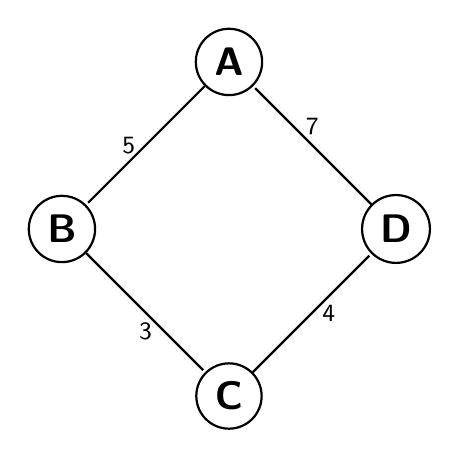
\begin{tikzpicture}[-,=stealth',shorten >=1pt,auto,node distance=3cm,
            thick,main node/.style={circle,draw,font=\sffamily\Large\bfseries}]

        \node[main node] (A) {A};
        \node[main node] (B) [below left of=A] {B};
        \node[main node] (C) [below right of=B] {C};
        \node[main node] (D) [below right of=A] {D};

        \path[every node/.style={font=\sffamily\small}]
        (A) edge node [left] {5} (B)
        (B) edge node [below] {3} (C)
        (C) edge node [right] {4} (D)
        (D) edge node [above] {7} (A);

    \end{tikzpicture}
\end{center}

Dans notre approche, chaque nœud du graphe représente ainsi une station spécifique, ou une borne de recharge et les arêtes du graphe représentent 
les connexions entre ces positions, et donc les routes même si nous avons supposé que nous travaillions en vol d'oiseau pour simplifier le problème.

L'utilisation des graphes nous permet de bénéficier d'algorithmes de recherche de chemins bien établis, tels que l'algorithme de Dijkstra que nous avons
étudié en cours de MSED ou l'algorithme A*, plus efficace mais aussi plus difficile à mettre en oeuvre. 

\subsubsection{Implémentation}
La structure Graph est composée de deux champs : V, qui représente le nombre de sommets du graphe, et adjMat, qui est une matrice d'adjacence représentant les arêtes du graphe. La matrice d'adjacence est un tableau à deux dimensions de taille V*(V+1)/2-V, où chaque élément est un entier représentant la pondération de l'arête correspondante. Si deux sommets ne sont pas connectés, la valeur de l'élément correspondant est -1 : \\

\begin{center}
    \begin{lstlisting}[caption=Structure du Graph]
typedef struct Graph {
    int V; 
    int* adjMat;
} Graph;
        \end{lstlisting}
\end{center}

\subsubsection{Spécification algébrique}

\begin{itemize}
    \item $createGraph : {Z} \rightarrow Graph^*$
    \item $printGraph : Graph^* \rightarrow void$
    \item $createGraphFromStations : ChargingStation^* \times {Z} \rightarrow Graph^*$
    \item $freeGraph : Graph^* \rightarrow void$
    \item $dijkstra : void^* \rightarrow void^*$
    \item $printPath : ChargingStation^* \times {Z}^* \times {Z} \times Coordinate^* \times Coordinate^* \rightarrow void$
    \item $serializeGraph : Graph^* \times char^* \rightarrow void$
    \item $deserializeGraph : char^* \times {Z} \rightarrow Graph^*$
\end{itemize}

\subsubsection{Parallélisation}

Afin de faciliter l'instanciation du graph, nous avons également mis en place une solution pour la création des arêtes du graph. En effet, la création des arêtes du graph est une opération coûteuse en temps, et nous avons donc décidé de la paraléliser. Pour cela, nous avons réalisé ces 2 structures additionnelles :

\begin{center}
    \begin{lstlisting}[caption=Structure Annexes à Graph]
typedef struct {
    ChargingStation* stations;
    int start;
    int end;
    Graph* graph;
} ThreadParamsGraph;

typedef struct {
    Graph* graph;
    ChargingStation* stations;
    int autonomy;
    int range;
    Coordinate* src;
    Coordinate* dest;
    int* n;
} ThreadParamsDijkstra;
\end{lstlisting}
\end{center}

La structure ThreadParamsGraph est conçue pour permettre le partage des paramètres nécessaires pour la création parallèle des arêtes du graphe. Elle contient un pointeur vers un tableau de stations de charge, des indices start et end définissant la plage de stations pour lesquelles le thread doit créer des arêtes, ainsi qu'un pointeur vers le graphe dans lequel les arêtes seront créées.

D'autre part, la structure ThreadParamsDijkstra est utilisée pour le partage des paramètres nécessaires à l'exécution parallèle de l'algorithme de Dijkstra. Elle contient un pointeur vers le graphe sur lequel l'algorithme doit être exécuté, un pointeur vers un tableau de stations de charge, ainsi que les paramètres autonomy et range utilisés dans l'algorithme. De plus, elle contient des pointeurs vers les coordonnées source et destination pour le chemin à trouver par l'algorithme de Dijkstra, ainsi qu'un pointeur vers un entier n qui stockera la longueur du chemin trouvé.

Ces structures permettent une modularité et une flexibilité accrue lors de la mise en place de la parallélisation dans le traitement du graphe, ce qui peut conduire à une amélioration significative des performances, en particulier pour les grands graphes.



\subsection{ChargingStation}

\subsubsection{Présentation}
La structure ChargingStation représente une station de recharge, avec des informations telles que le nom de la station, les coordonnées géographiques, le nombre de points de charge et le nombre de points de charge disponibles. Elle contient également une file d'attente pour gérer les véhicules en attente de recharge. Les ChargingStation sont utilisés comme noeuds du graphe :

\begin{center}
    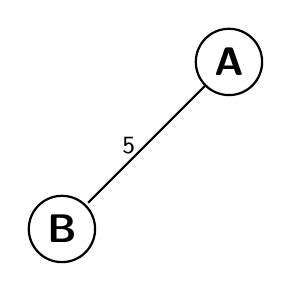
\begin{tikzpicture}[-,=stealth',shorten >=1pt,auto,node distance=3cm,
            thick,main node/.style={circle,draw,font=\sffamily\Large\bfseries}]

        \node[main node] (A) {A};
        \node[main node] (B) [below left of=A] {B};

        \path[every node/.style={font=\sffamily\small}]
        (A) edge node [left] {5} (B);

    \end{tikzpicture}
\end{center}

\subsubsection{Implémentation}
La structure ChargingStation est composée de cinq champs : name, qui est un pointeur vers une chaîne de caractères contenant le nom de la station, coord, qui est un pointeur vers une structure Coordinate contenant les coordonnées géographiques de la station, nbChargingPoints, qui est un entier représentant le nombre de points de charge de la station, nbAvailableChargingPoints, qui est un entier représentant le nombre de points de charge disponibles, et queues, qui est un tableau de pointeurs vers des files d'attente, une pour chaque point de charge. \\

\begin{center}
    \begin{lstlisting}[caption=Structure ChargingStation]
typedef struct ChargingStation {
    char* name;
    Coordinate* coord;
    int nbChargingPoints;
    int nbAvailableChargingPoints;
    Queue** queues ;
} ChargingStation;
        \end{lstlisting}
\end{center}

\subsubsection{Spécification algébrique}

\begin{itemize}
    \item $readJSONstations : char^* \times {Z} \rightarrow ChargingStation^*$
    \item $serializeStations : char^* \times ChargingStation^* \times {Z} \rightarrow void$
    \item $deserializeStations : char^* \times {Z} \rightarrow ChargingStation^*$
    \item $addPersonToStation : ChargingStation^* \times Person^* \times {Z} \times {Z} \rightarrow void$
    \item $removePersonFromStation : ChargingStation^* \times Person^* \rightarrow void$
    \item $getBestQueue : ChargingStation^* \rightarrow Queue^*$
\end{itemize}


\subsection{Queue}

\subsubsection{Présentation}
La structure Queue est utilisée pour gérer la liste des véhicules en attente de recharge à une station donnée. Elle est basée sur une liste doublement chaînée, qui permet des opérations d'ajout et de suppression efficaces à la fois en tête et en queue de liste :

\begin{center}
    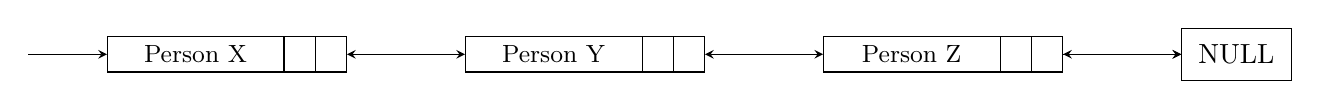
\begin{tikzpicture}[
            list/.style={rectangle split, rectangle split parts=3,
                    draw, rectangle split horizontal,minimum width=2cm,text width=2cm,
                    text centered, font=\small},
            >=stealth, start chain,
            node distance=1.5cm,
            every on chain/.style={join},
            every join/.style={<->}]

        \node[list,on chain] (A) {Person X};
        \node[list,on chain] (B) {Person Y};
        \node[list,on chain] (C) {Person Z};
        \node[on chain,draw,inner sep=6pt] (D) {NULL};

        \draw[<-] (A.one west) -- ++(-1cm,0);
        \draw[->] (C.three east) -- (D);
    \end{tikzpicture}
\end{center}

\subsubsection{Implémentation}
La structure Queue est composée de trois champs : data, qui est un pointeur vers une structure Person contenant les informations sur le véhicule en attente, next, qui est un pointeur vers la file d'attente suivante, et prev, qui est un pointeur vers la file d'attente précédente. \\

\begin{center}
    \begin{lstlisting}[caption=Structure Queue]
typedef struct Queue {
    Person* data;
    struct Queue* next;
    struct Queue* prev;
} Queue;
    \end{lstlisting}
\end{center}


\subsubsection{Spécification algébrique}
\begin{itemize}
    \item $createQueue : void \rightarrow Queue^*$
    \item $del\_person : Queue^* \rightarrow void$
    \item $push : Queue^* \times Person^* \times {Z} \rightarrow void$
    \item $last : Queue^* \rightarrow Person^*$
    \item $index\_of\_from : Queue^* \times {Z} \rightarrow Person^*$
    \item $timeToWait : Queue^* \rightarrow {Z}$
    \item $first : Queue^* \rightarrow Person^*$
    \item $pop : Queue^* \rightarrow void$
\end{itemize}

\section{Fonctionnalités et algorithmes}
\subsection{Algorithme de Dijkstra}
\subsubsection{Présentation}
Pour déterminer le parcours optimal d'une station à une autre, nous avons utilisé l'algorithme de Dijkstra. C'est un choix naturel pour ce problème, 
car il trouve le chemin le plus court entre deux sommets d'un graphe pondéré, ce qui est exactement ce dont nous avons besoin pour minimiser 
la distance de conduite et donc la consommation d'énergie. Nous avons également exploré un potentiel choix alternatif, l'algorithme A*. Cependant, en 
raison des contraintes de temps liés au projet, nous avons finalement décidé de nous en tenir à l'algorithme de Dijkstra qui est celui vu en cours de 
MSED, mais en implémentant une version parallèle pour améliorer les performances, et également 
en retirant un grand nombre de sommets du graphe pour réduire le temps d'exécution.

\subsubsection{Analyse de compléxité}

La complexité de l'algorithme de Dijkstra est en général de $O(V^2)$, où $V$ est le nombre de sommets du graphe. Cependant, si le graphe est implémenté à l'aide d'une liste d'adjacence et d'une file de priorité, la complexité peut être réduite à $O((V+E) log V)$, où E est le nombre d'arêtes. Dans notre cas, nous avons utilisé une matrice d'adjacence pour représenter le graphe, donc la complexité est de $O(V^2)$. Cependant, nous avons également utilisé une version parallèle de l'algorithme, qui réduit considérablement le temps d'exécution. En effet, l'algorithme de Dijkstra est composé de deux boucles imbriquées, et la boucle interne peut être parallélisée, ce qui permet d'obtenir une complexité de $O(V^2/p)$, où $p$ est le nombre de threads utilisés. En outre, nous avons également réduit le nombre de sommets du graphe, ce qui réduit encore le temps d'exécution.

\subsection{Instanciation du Graph}

\subsubsection{Load des stations}
Pour instancier le graphe, nous avons besoin de charger les stations de charge depuis un fichier JSON. Pour cela, nous avons utilisé la bibliothèque cJSON, qui permet de lire et d'écrire des fichiers JSON en C. Nous avons créé une fonction readJSONstations qui prend en paramètre le nom du fichier JSON et le nombre de stations à load, et qui renvoie un tableau de stations de charge. Cette fonction utilise la bibliothèque cJSON pour lire le fichier JSON et créer un tableau de stations de charge à partir des données du fichier. Elle renvoie ensuite ce tableau.

\subsubsection{Instanciation de la matrice d'adjacence}
Une fois les stations de charge instanciées, nous pouvons instancier la matrice d'adjacence. Pour cela, nous avons créé une fonction createGraphFromStations qui prend en paramètre un tableau de stations de charge et le nombre de stations, et qui renvoie un graphe. Cette fonction crée un graphe vide, puis crée les arêtes du graphe en utilisant la fonction createGraphFromStations. Enfin, elle renvoie le graphe.

\subsubsection{Analyse de compléxité}
La fonctionnalité d'instanciation du graphe est composée de deux fonctions majeures : createGraphFromStations et createGraphFromStationsThread.

createGraphFromStationsThread est une fonction qui remplit une partie de la matrice d'adjacence du graphe. En particulier, chaque thread exécute deux boucles imbriquées, où l'index i varie de start à end - 1 et l'index j varie de i + 1 à end. Par conséquent, cette partie a une complexité de $O((end-start)^2)$. Dans le cas le plus équilibré, chaque thread doit gérer $n / numThreads$ sommets, ce qui donnerait une complexité d'environ $O((n / numThreads)^2)$ pour chaque thread.

Cependant, l'aspect important de la parallélisation est que les threads s'exécutent simultanément. Par conséquent, bien que chaque thread individuel puisse avoir une complexité de $O((n / numThreads)^2)$, l'ensemble de l'opération createGraphFromStations a une complexité approximative de $O((n / numThreads)^2)$.

Il est à noter que l'efficacité de la parallélisation dépend de nombreux facteurs, dont la disponibilité des ressources du système, la gestion des threads par le système d'exploitation et la concurrence d'accès aux ressources partagées. Par conséquent, dans la pratique, le gain de performances peut ne pas être aussi important que suggéré par cette analyse.

En ce qui concerne la complexité spatiale, chaque thread n'utilise que très peu de mémoire supplémentaire (juste quelques variables locales). Ainsi, la complexité spatiale globale est dominée par la taille du graphe, qui est $O(n^2)$, où n est le nombre de sommets (stations) dans le graphe, car nous utilisons une matrice d'adjacence pour représenter le graphe.

\subsection{Visualisation d'itinéraires}

\subsubsection{Présentation}

Afin de visualiser le parcours trouvé lors de l'exécution de l'algorithme de Dijkstra, nous avons fait appel à une fonctionnalité de Google Maps, permettant de relier des coordonnées entre elles. Ainsi, nous générons une URL Google Maps, qui prend en paramètre chaque étape du parcours. Celle-ci est ensuite ouverte dans le navigateur par défaut de l'utilisateur et affiche le parcours.

\subsection{Mode simulation}
\subsubsection{Présentation}
Le mode simulation permet de simuler le comportement de plusieurs véhicules électriques en circulation. Ce mode permet d'instancier un grand nombre de $Person$, qui correspondent aux "automobilistes". Le mode simulation permet de leur attribuer des destinations et de les faire circuler dans le réseau. Le mode simulation permet également de simuler le temps de recharge des véhicules, en fonction de leur autonomie et de leur niveau de charge actuel. Nous avons également implémenté un système de queue pour gérer les véhicules en attente de recharge.


\section{Tests}

\subsection{Introduction}
Nous avons effectué des tests sur chacune de nos fonctions pour nous assurer qu'elles fonctionnent correctement. Ces tests comprenaient des cas de test simples ainsi que des tests de stress pour évaluer la performance et l'efficacité des fonctions. En outre, nous avons utilisé des outils d'analyse dynamique pour détecter les fuites de mémoire et autres problèmes liés à la gestion de la mémoire.

\subsubsection{Exemple}

\begin{center}
    \begin{figure}[H]
        \centering
        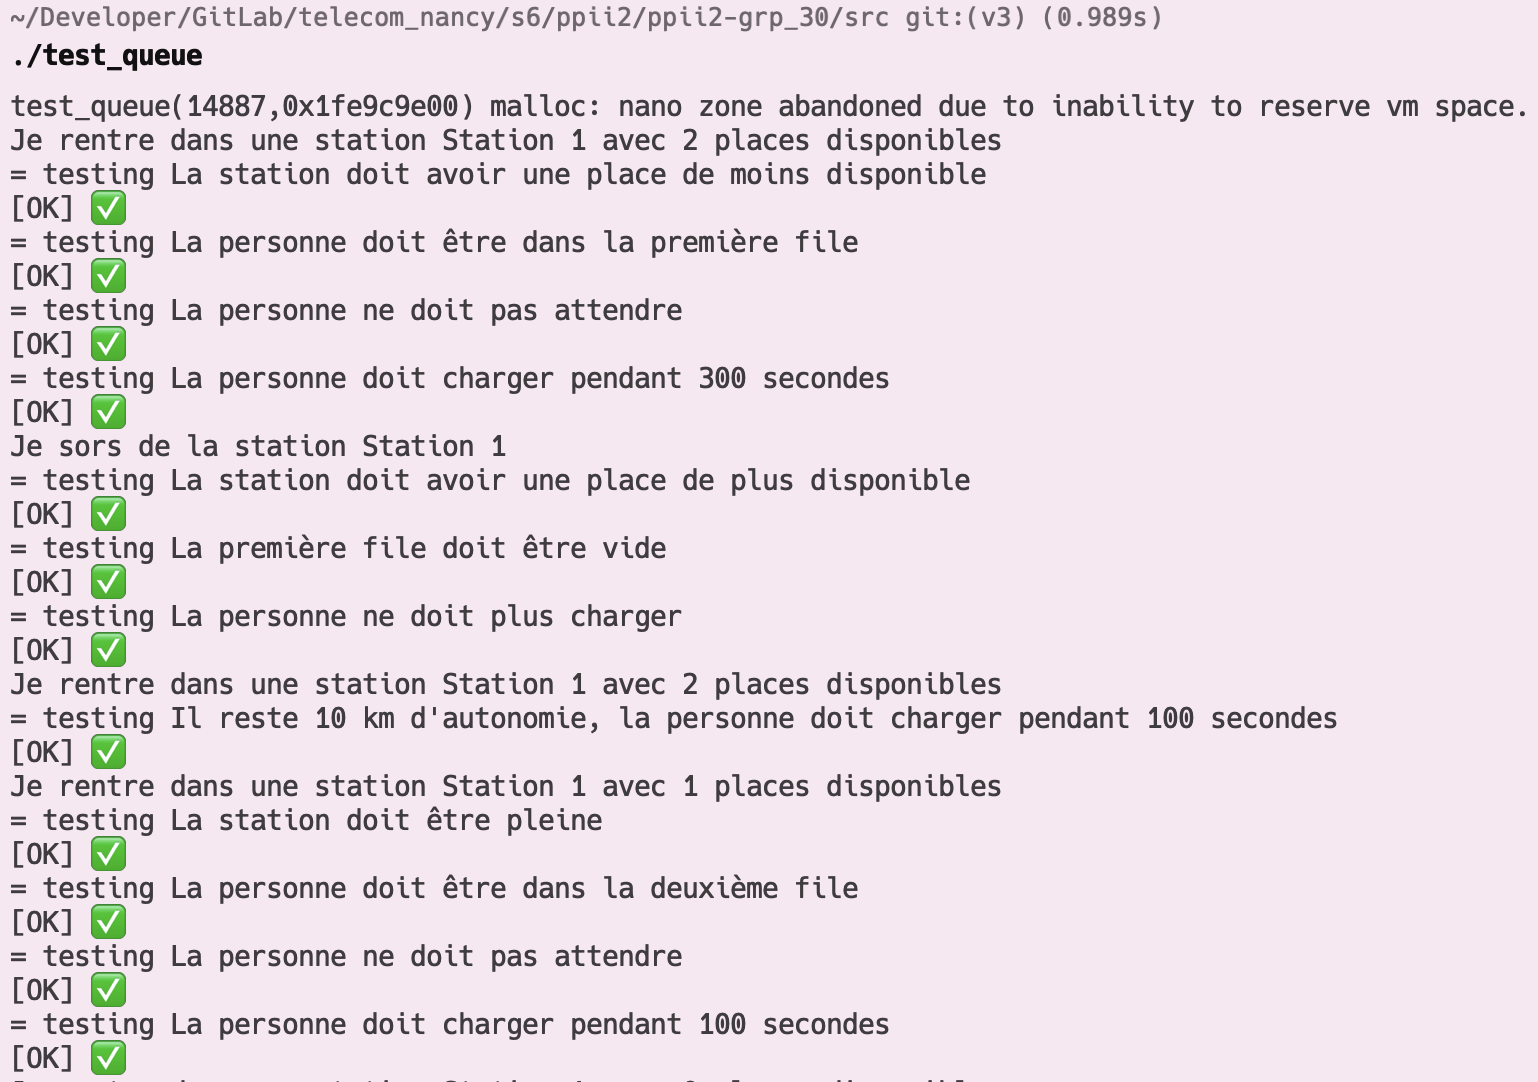
\includegraphics[width=0.75\textwidth]{img/TEST.png}
        \caption{Sortie Console}
    \end{figure}
\end{center}

\section{Gestion de projet}
\subsection{Équipe de projet}
Ce projet est un projet local réalisé en groupe de 4 personnes~:
\begin{itemize} 
    \item Alexis MARCEL
    \item Lucas LAURENT
    \item Noé STEINER
    \item Mathias AURAND-AUGIER
\end{itemize}
Le comité de pilotage est constitué de~:
\begin{itemize}
    \item Anne-Claire HEURTEL
    \item Olivier FESTOR
    \item Gérald OSTER
\end{itemize}
Ces personnes constituent les parties prenantes de notre projet ainsi que les acteurs influents sur le livrables.
\begin{figure}[H]
    \centering
    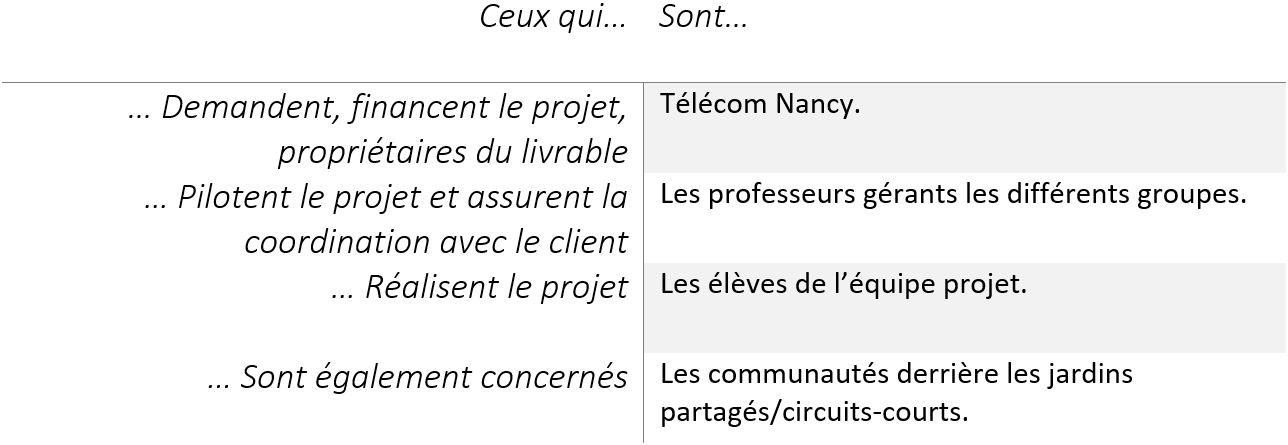
\includegraphics[width=0.75\textwidth]{img/parties_prenantes.png}
    \caption{Parties prenantes}
\end{figure}
\subsection{Organisation au sein de l’équipe projet}
Nous avons réalisé plusieurs réunions, en présentiel dans les locaux de Télécom Nancy mais la plupart de notre collaboration a eu lieu sur Discord. Ces réunions nous ont permis de mettre en commun nos avancées régulièrement, de partager nos connaissances sur des problématiques et de nous organiser de manière optimale.
En plus des réunions d'avancement régulières, nous avons également réalisé des réunions techniques afin de résoudre un problème ou bien de réfléchir à la conception.
Les comptes rendus des réunions réalisées sont présents dans l’\hyperlink{annexe1}{Annexe 1}.

Contrairement au premier projet, nous avons choisi de travailler cette fois-ci tous ensemble plutôt qu'individuellement. Nous avons donc utilisé une 
application pour que nous puissions tous modifier le code en même temps, ce qui nous a permis de tous travailler sur le même code en même temps.

Ensuite, nous avons utilisé GitLab pour gérer les différentes versions du développement de notre application, ainsi que les différentes 
branches nous permettant de travailler simultanément sans conflit.

Enfin, la rédaction des differents comptes rendus de réunion et des rapports ont été rédigé en \LaTeX.

\subsection{Objectifs SMART}
La méthode SMART que l'on rappelle ci-dessous nous a permis de définir nos différents objectifs :

\begin{figure}[H]
    \centering
    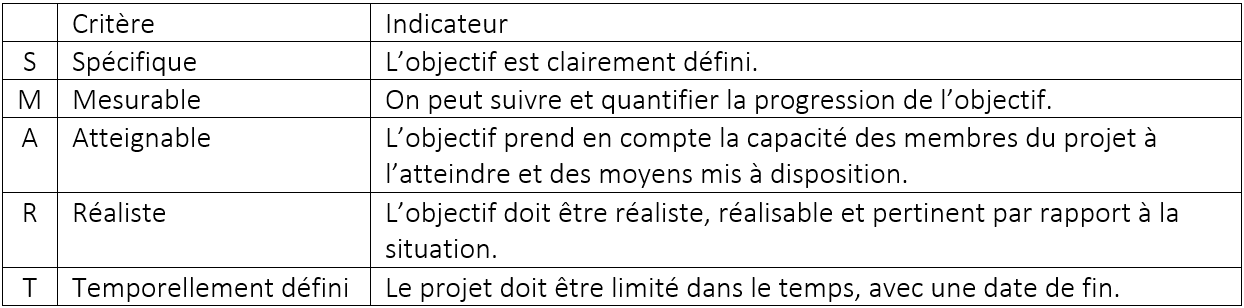
\includegraphics[width=1\textwidth]{img/SMART.png}
    \caption{Objectifs SMART}
\end{figure}

\subsection{Matrice des objectifs}
Nous avons conçu, à l'aide de la méthode SMART, la matrice des objectifs suivante :

\begin{figure}[H]
    \centering
    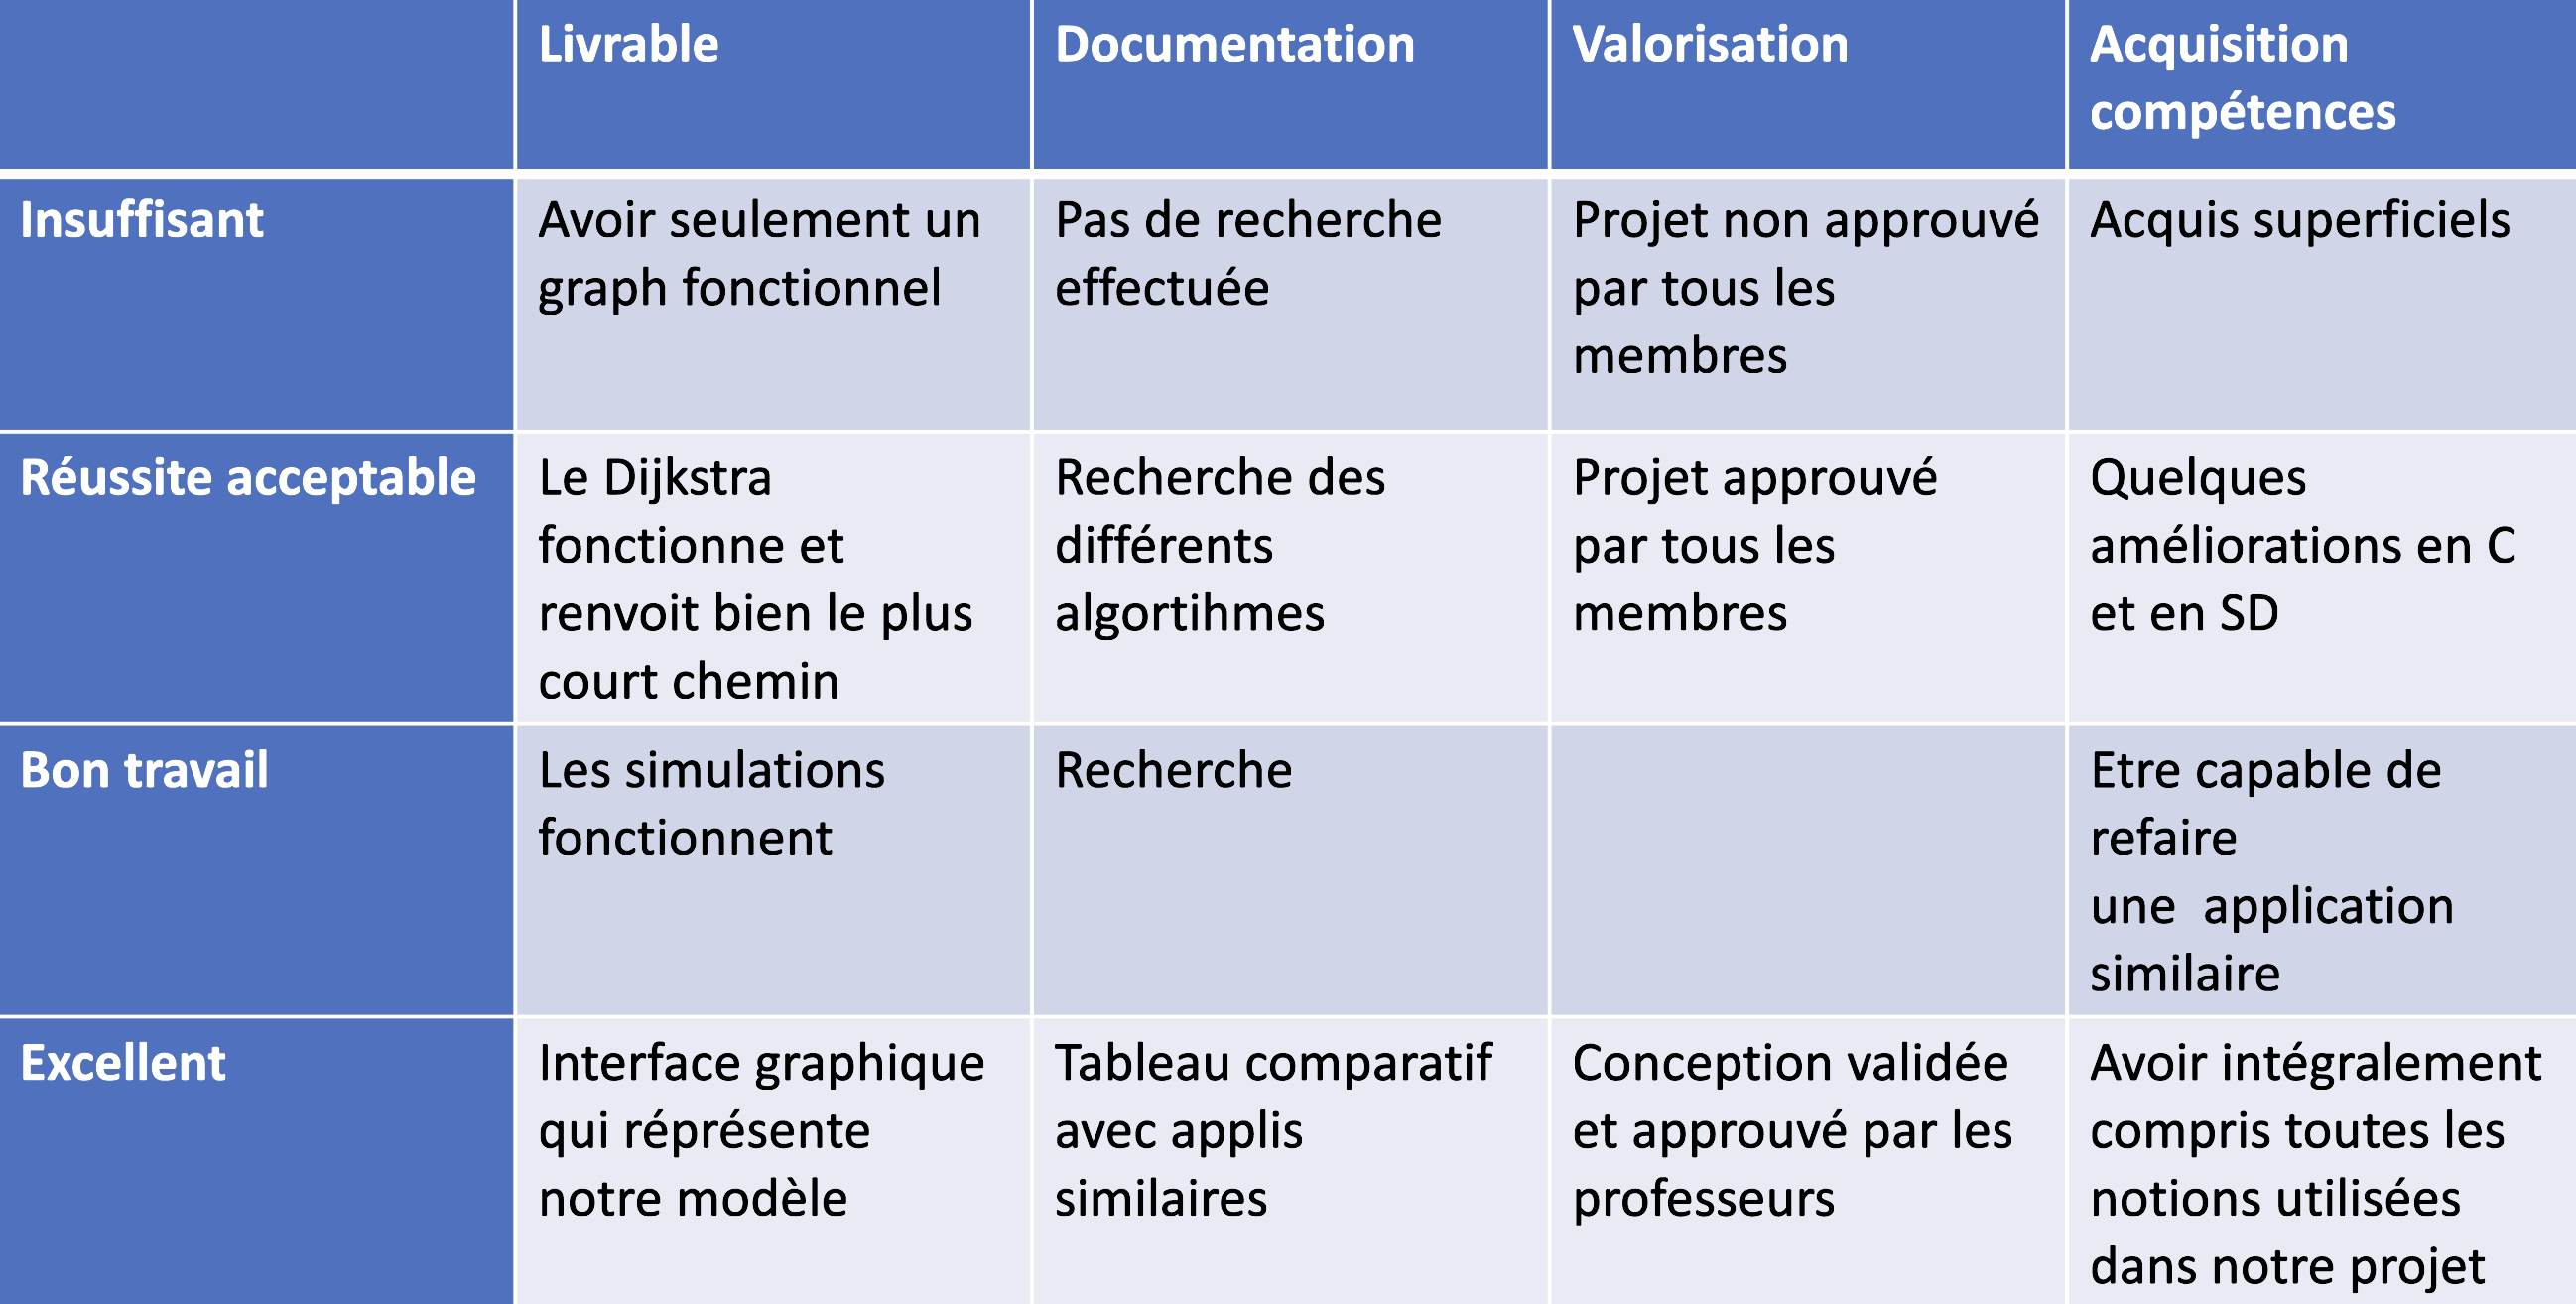
\includegraphics[width=1\textwidth]{img/matrice_des_objectifs.png}
    \caption{Matrice des objectifs}
\end{figure}

En ce qui concerne, le livrable, il sera difficile, compte tenu des délais d'attendre tous les objectifs du projet.
\subsection{Triangle qualité-cout-délai}
Afin d’établir des objectifs cohérents, et réalisables dans les délais, nous avons réalisé le triangle qualité-coût-délai. On remarque ainsi, les délais étant courts, que nous avons tout intérêt à ne pas se fixer des objectifs trop ambitieux sous peine de devoir renoncer à certaines fonctionnalités et de ne pas rendre le livrable annoncé initialement.

\begin{figure}[H]
    \centering
    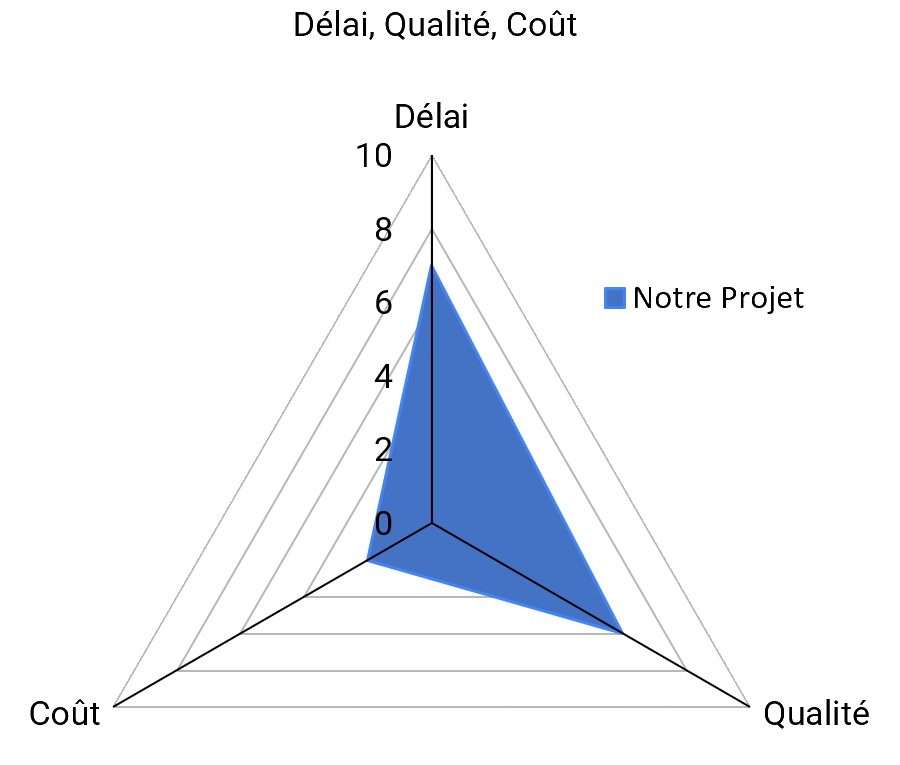
\includegraphics[width=0.5\textwidth]{img/triangle_QCD.png}
    \caption{Triangle DQC}
\end{figure}

\subsection{Matrice SWOT}
Afin d’avoir une vision plus globale de nos ressources et des facteurs internes et externes agissant sur le projet, nous avons ensuite réalisé la matrice SWOT (Strengths, Weaknesses, Opportunities, Threats) de notre projet.

\begin{figure}[H]
    \centering
    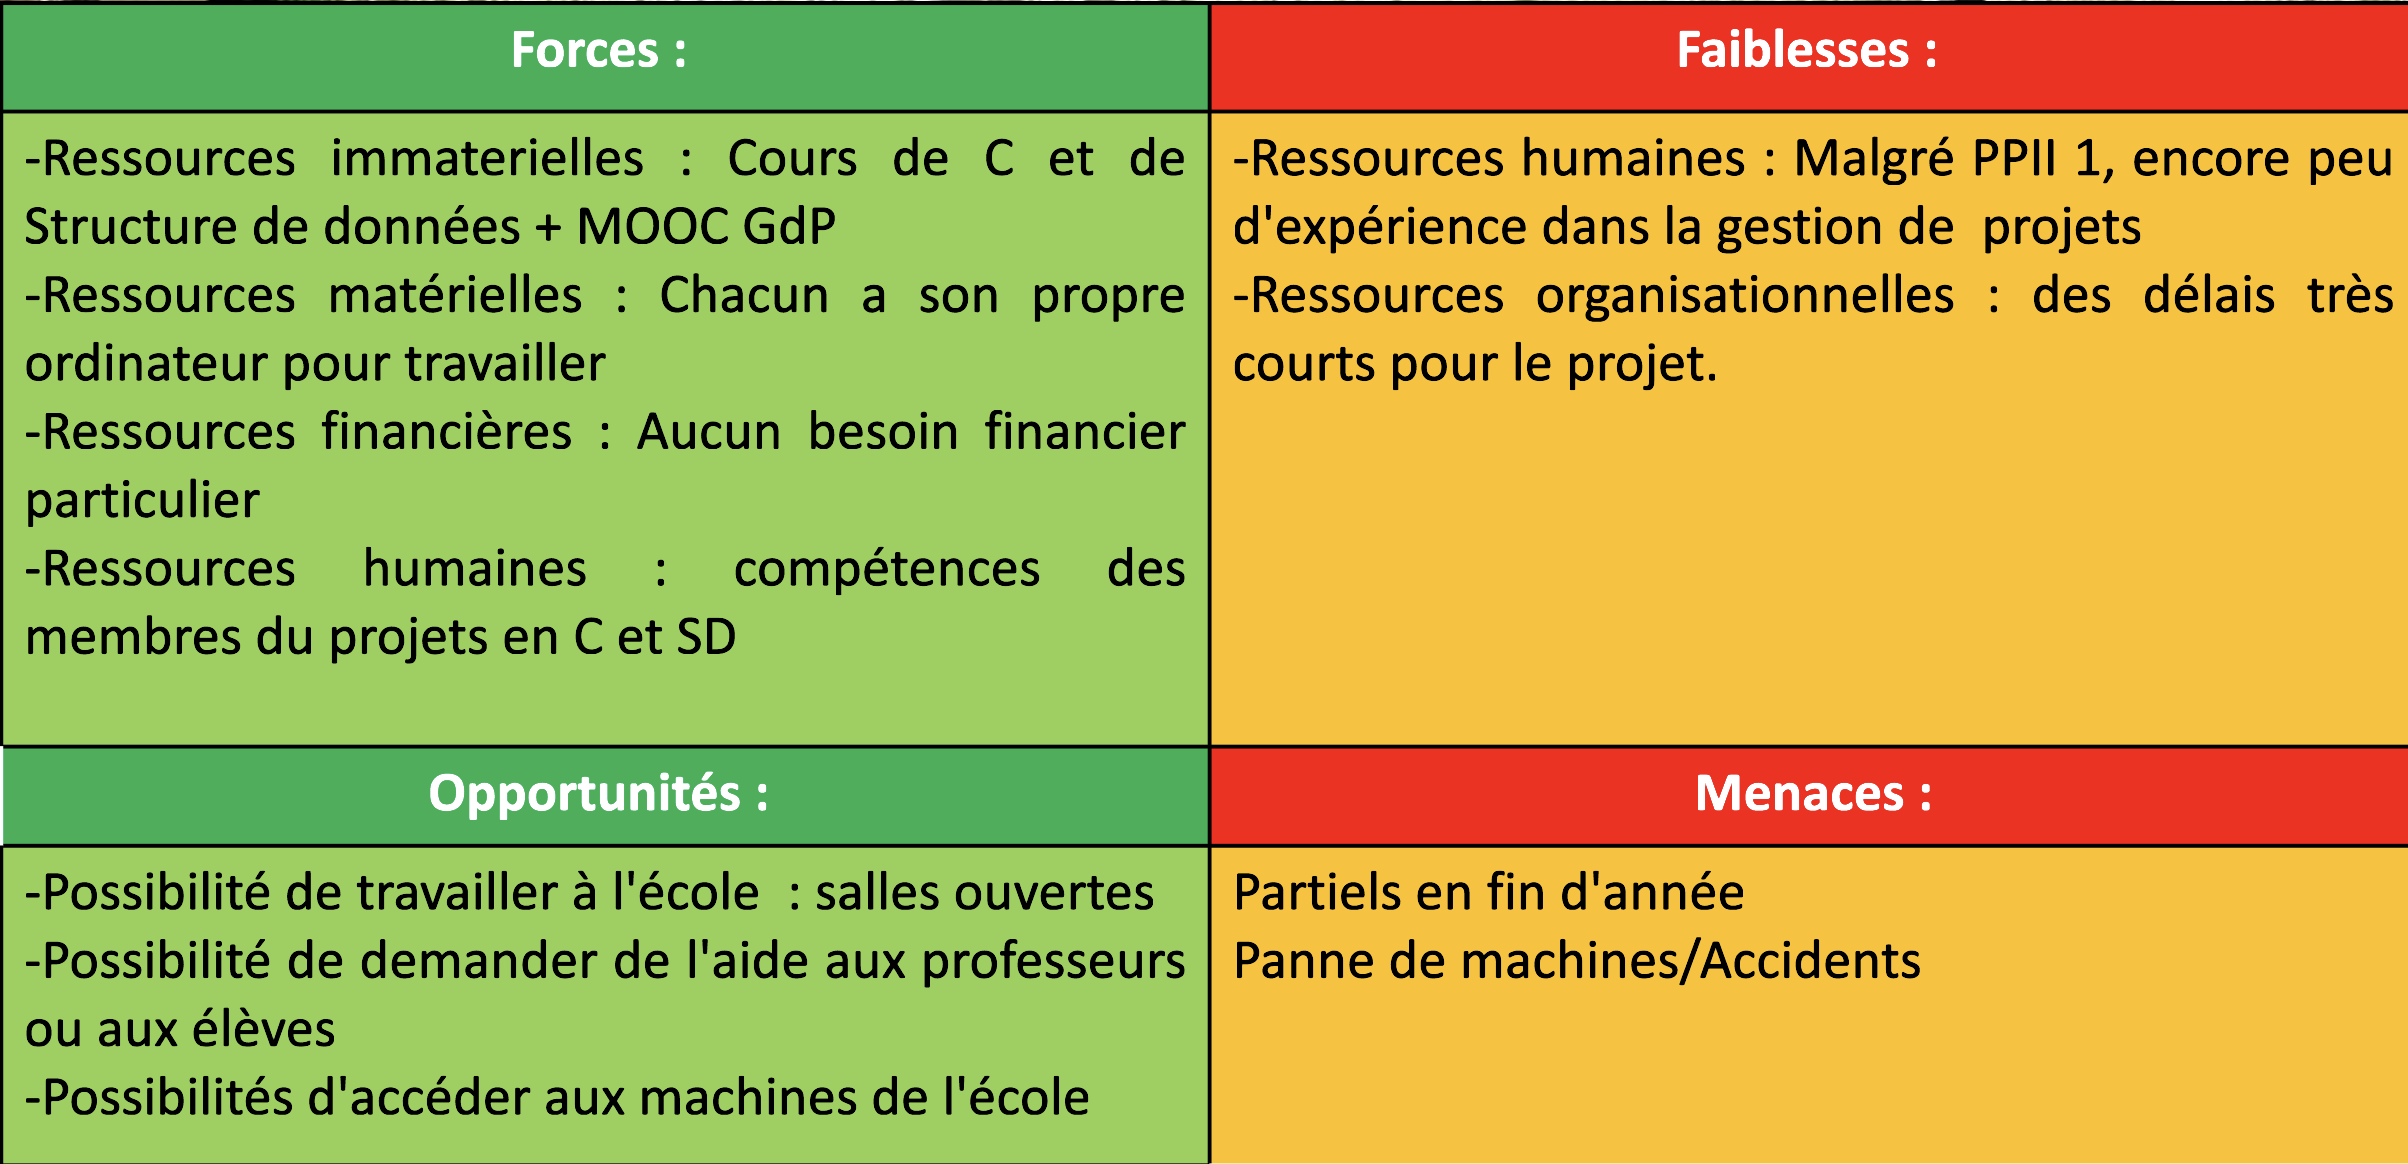
\includegraphics[width=0.75\textwidth]{img/SWOT.png}
    \caption{Matrice SWOT}
\end{figure}

On peut ainsi remarquer que notre projet présente de nombreux points forts notamment grâce aux connaissances acquises lors des cours de Télécom Nancy 
mais également de par l’expérience forte de deux des membres de l’équipe projet.  Cependant, plusieurs facteurs internes constituent nos faiblesses
 notamment les courts délais qui nous obligent à être concis et efficaces dans notre travail. Cependant, nous avons également des opportunités notamment 
 celle de pouvoir demander de l'aide aux autres élèves et aux professeurs, ou encore le fait que les salles soient ouvertes et à notre disposition pour
 les réunions de groupe.

De plus, nous devons anticiper les charges de travail dans le cadre de notre formation à Télécom Nancy qui s'avèrent être plus élevées au mois de mai 
pour les partiels de fin d'année. Nous allons donc devoir prendre cela en compte dans notre gestion des tâches.

\subsection{Profil de projet}

Afin d’avoir une vision plus globale sur notre projet, nous avons également réalisé le profil du projet (le budget étant égal à 0, nous avons choisi de ne pas le représenter dans notre profil). On remarque que, du fait des nombreuses fonctionnalités que nous avons l’intention d’implémenter dans notre application, que notre projet est de taille moyenne mais de complexité élevée.

Cependant, les enjeux du projet ne sont pas très importants (en dehors de la note finale qui compte dans notre moyenne) car l'échec du projet n'engendrera pas la chute d'une organisation et le budget est négligeable.

De plus, au vu de l’état de l’art établi, l’innovation du projet est importante puisque peu d'application de ce type existent actuellement.

\begin{figure}[H]
    \centering
    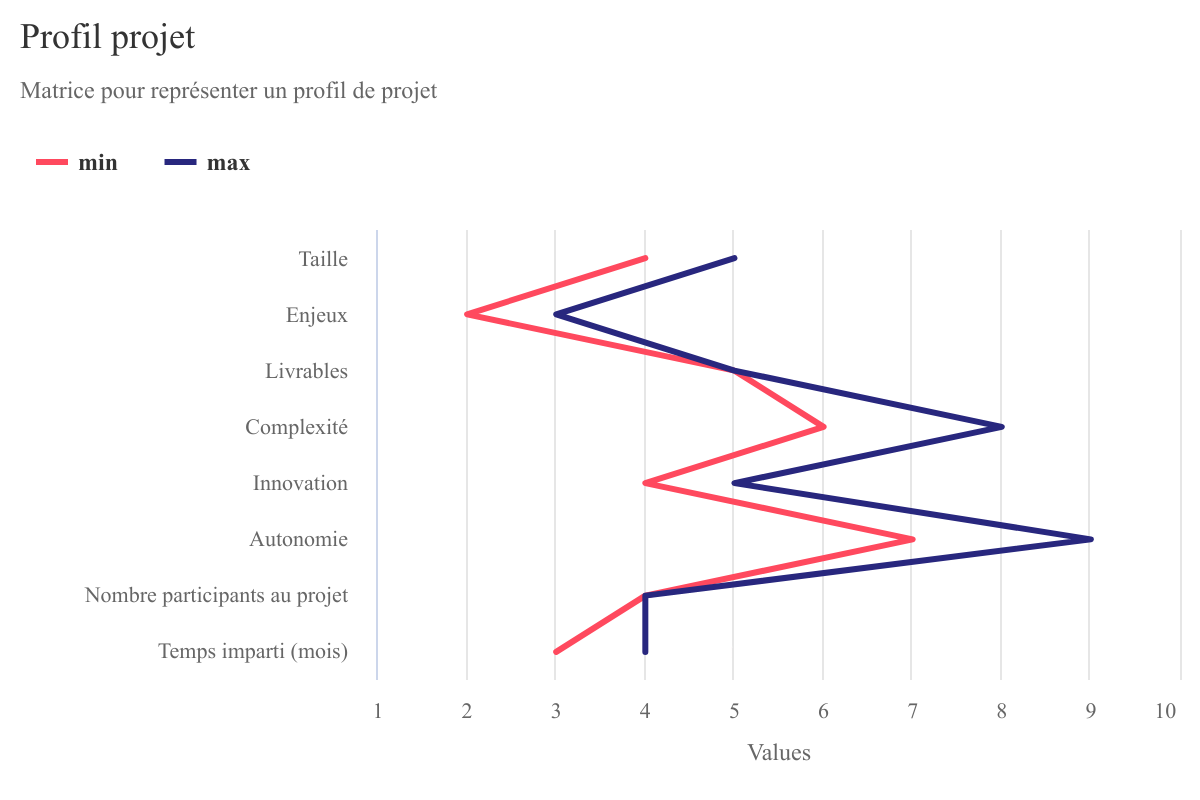
\includegraphics[width=0.75\textwidth]{img/profil_projet.png}
    \caption{Profil du projet}
\end{figure}

\subsection{WBS~: comment concrétiser l’application}
Ceci étant fait, nous avons maintenant choisi de détailler les lots de travail à effectuer pour fabriquer notre application. Nous avons ainsi réalisé le WBS (Work Breakdown Structure) de notre application~: il apparait ainsi les grandes étapes de notre projet que sont~: définition du cadre de l’application, développement des fonctionnalités de l’application et écriture du rapport.
\begin{figure}[H]
    \centering
    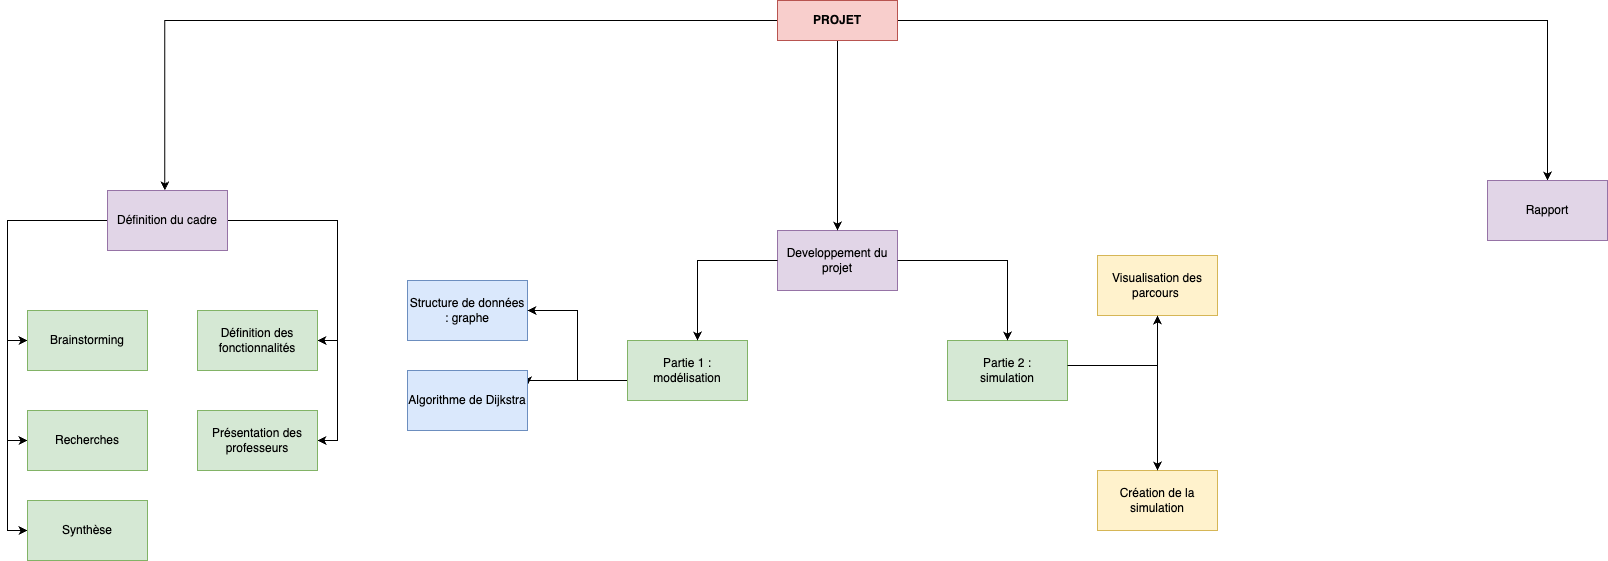
\includegraphics[width=1\textwidth]{img/WBS.png}
    \caption{WBS}
\end{figure}

\subsection{Diagramme de Gantt~: planification}
Maintenant que nous avons un détail des lots de travail qui constituent notre application, il faut maintenant les mettre en relation pour créer un planning efficace où chaque tâche est effectuée dans l’ordre.
\begin{figure}[H]
    \centering
    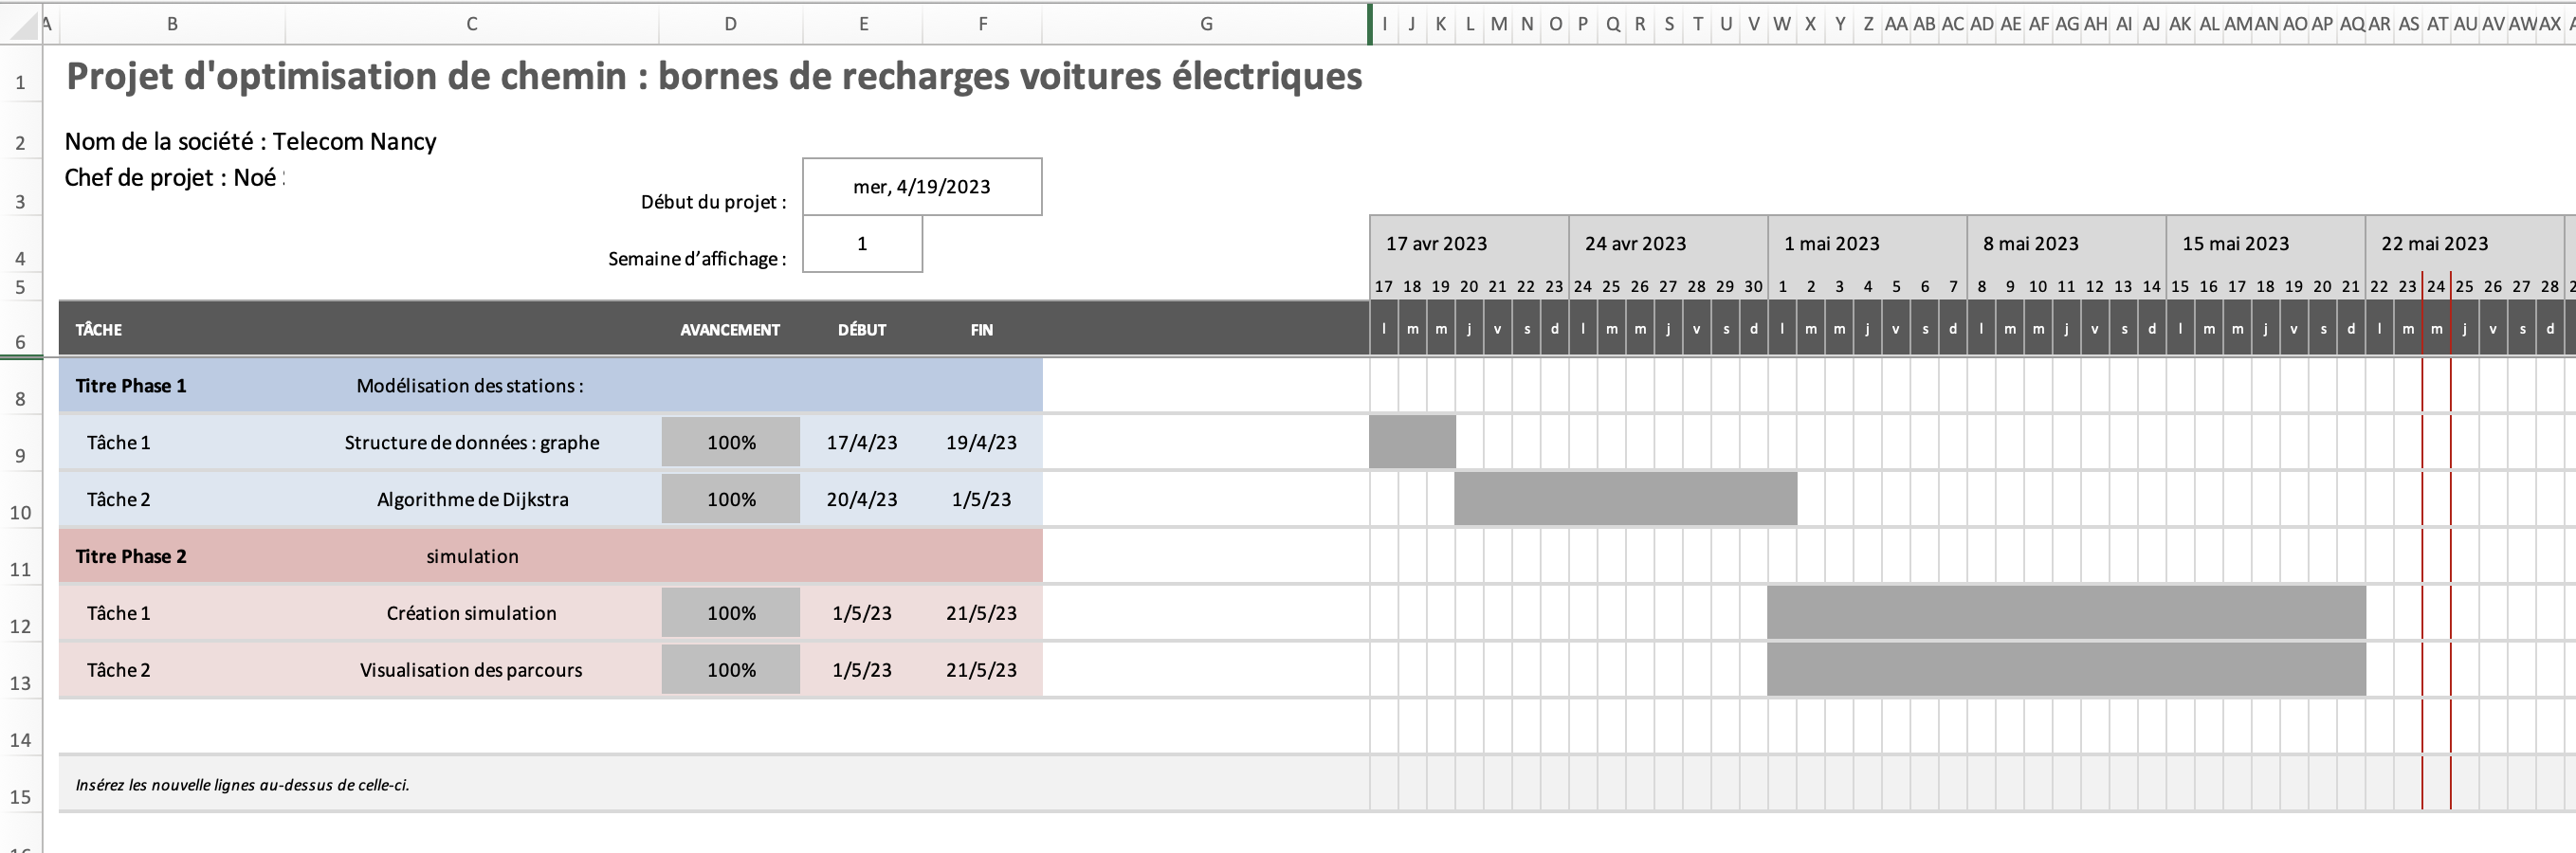
\includegraphics[width=1\textwidth]{img/gantt.png}
    \caption{Diagramme de GANTT}
\end{figure}
Ce diagramme est une première version générale des tâches à effectuer, il sera modifié et détaillé davantage une fois la conception et les maquettes du projet réalisées.

\subsection{Matrice RACI}
Nous avons choisi de ne pas faire de matrice RACI à cause des choix d'organisation que nous avons faits. En effet, 
nous avons décidé de travailler en groupe sur toutes les tâches, ce qui fait que nous sommes tous responsables de toutes les tâches et qu'il n'y a, de ce fait, 
pas de répartition précise des tâches.

\subsection{Gestion des risques}
Nous avons également pensé à prévoir une partie des risques pouvant se dresser sur notre route, les risques les plus classiques étant
la gestion du temps et le manque de compréhension de certaines personnes de l'équipe.
\begin{figure}[H]
    \centering
    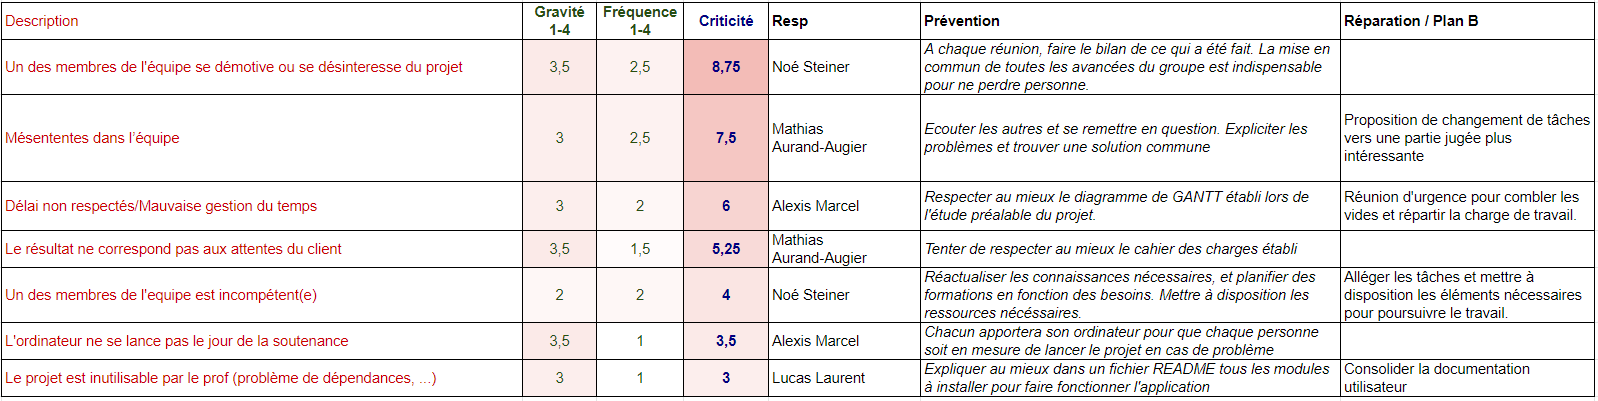
\includegraphics[width=1\textwidth]{img/Plan_gestion_risque.png}
    \caption{Plan de gestion des risques}
\end{figure}

\section{Conclusion}

En conclusion, ce projet s'est révélé être une expérience d'apprentissage extrêmement précieuse, nous permettant d'affiner et de développer nos compétences en programmation en langage C. Nous avons approfondi notre compréhension des structures de données, notamment comment les utiliser efficacement pour manipuler, stocker et accéder aux informations. Ce projet nous a aussi donné l'opportunité d'appliquer des algorithmes complexes, comme celui de Dijkstra, dans un contexte réel, nous permettant d'apprécier l'importance de ces outils dans la résolution de problèmes concrets.
\newline
En travaillant sur un problème réel - l'optimisation du placement des stations de charge pour véhicules électriques - nous avons pu saisir l'importance des implications de notre travail. Cela a ajouté une dimension plus large à notre apprentissage, en nous faisant comprendre comment les compétences techniques que nous avons acquises peuvent avoir un impact sur des questions d'une grande pertinence sociétale, comme la transition vers une mobilité plus durable.
\newline
De plus, la mise en évidence des enjeux de l'énergie durable dans notre projet nous a permis de nous immerger dans un secteur d'une importance cruciale pour l'avenir de notre société. L'efficacité de la distribution de l'énergie, en particulier pour les véhicules électriques, est une question clé dans la lutte contre les changements climatiques. En participant à la résolution de ce problème à travers notre projet, nous avons non seulement appliqué nos compétences techniques, mais également contribué à un domaine qui aura un impact durable et positif sur notre avenir.
\newline
En somme, ce projet nous a offert une occasion inestimable de croissance personnelle et professionnelle. Il nous a permis d'acquérir et de consolider des compétences techniques, tout en nous faisant prendre conscience de l'importance des implications de notre travail dans le monde réel, en particulier dans le domaine de la mobilité et de l'énergie durables.

\section{Annexes}
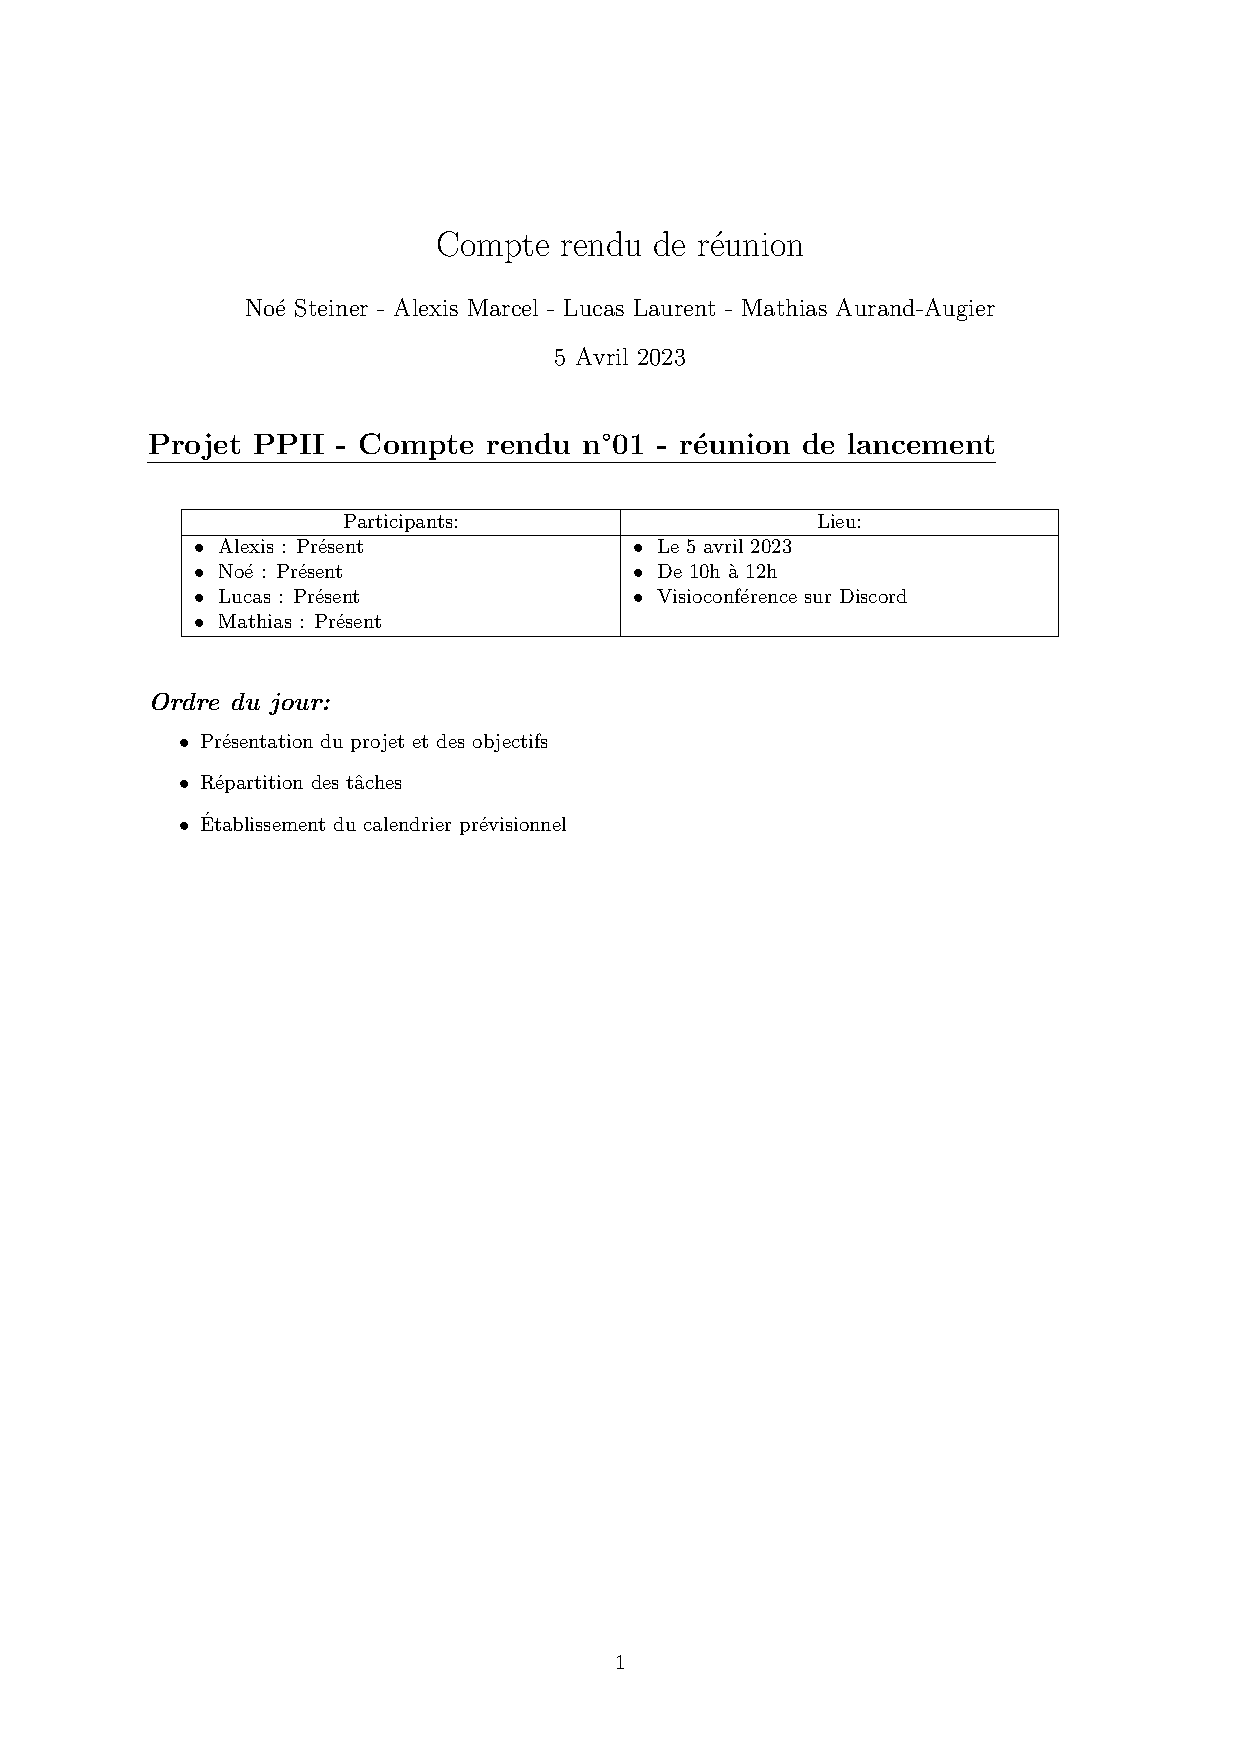
\includepdf[pages=1]{../cr_reu/reu1/cr_reu1.pdf}
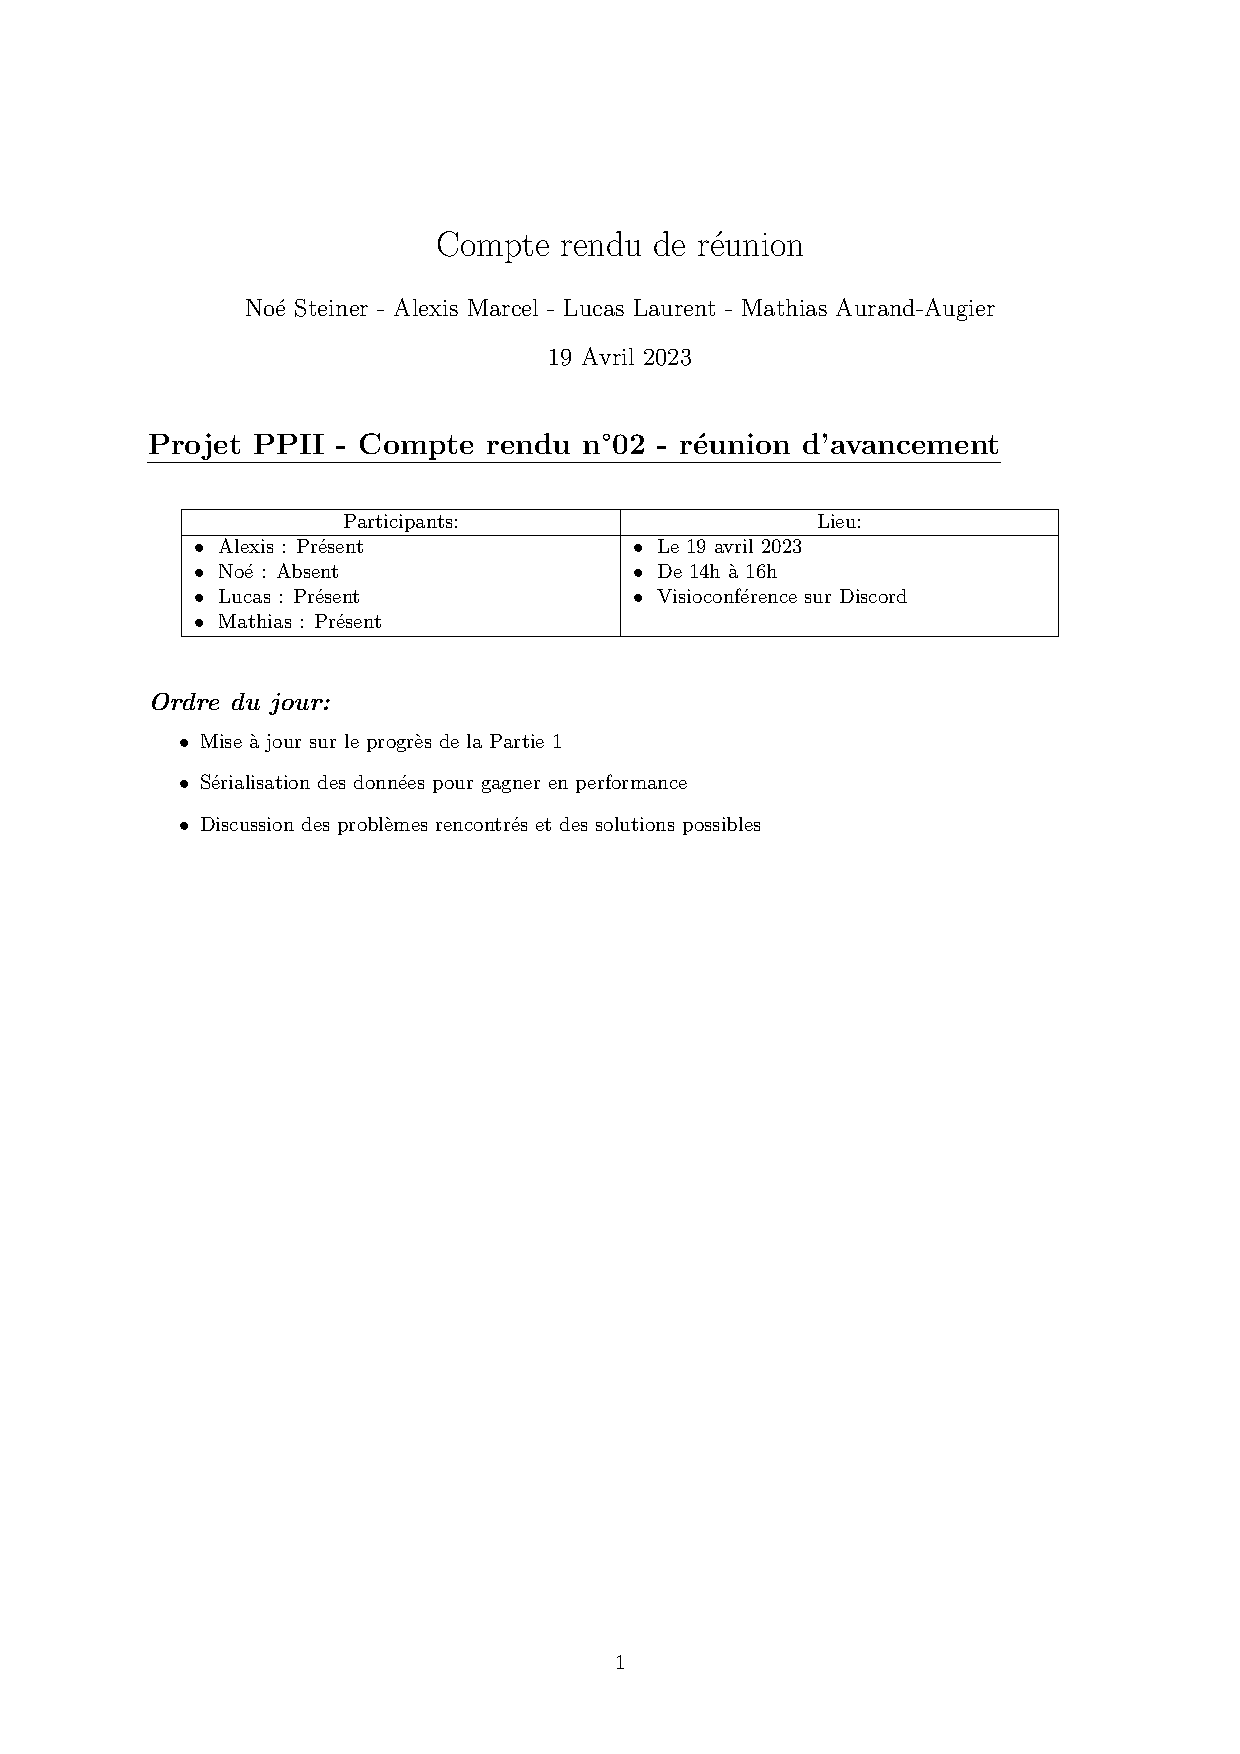
\includepdf[pages=1]{../cr_reu/reu2/cr_reu2.pdf}
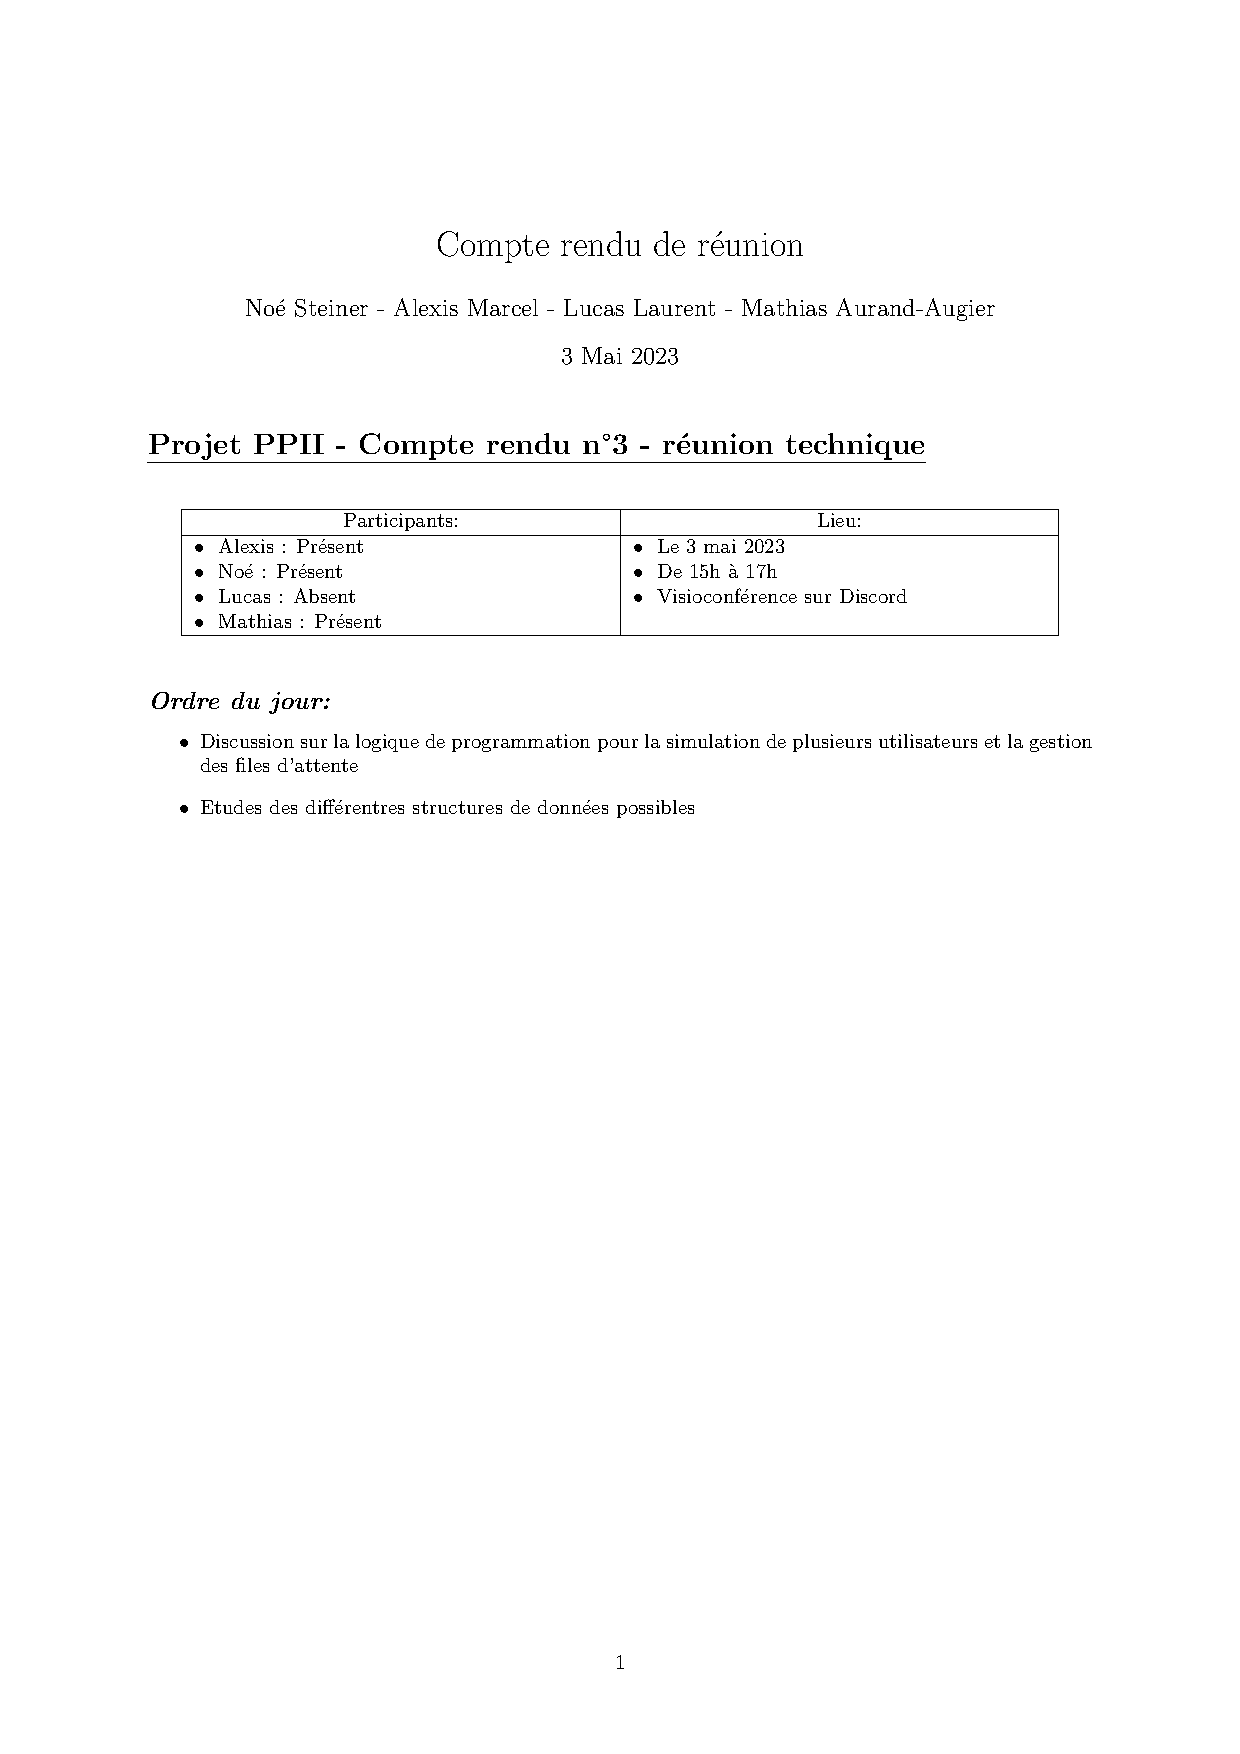
\includepdf[pages=1]{../cr_reu/reu3/cr_reu3.pdf}
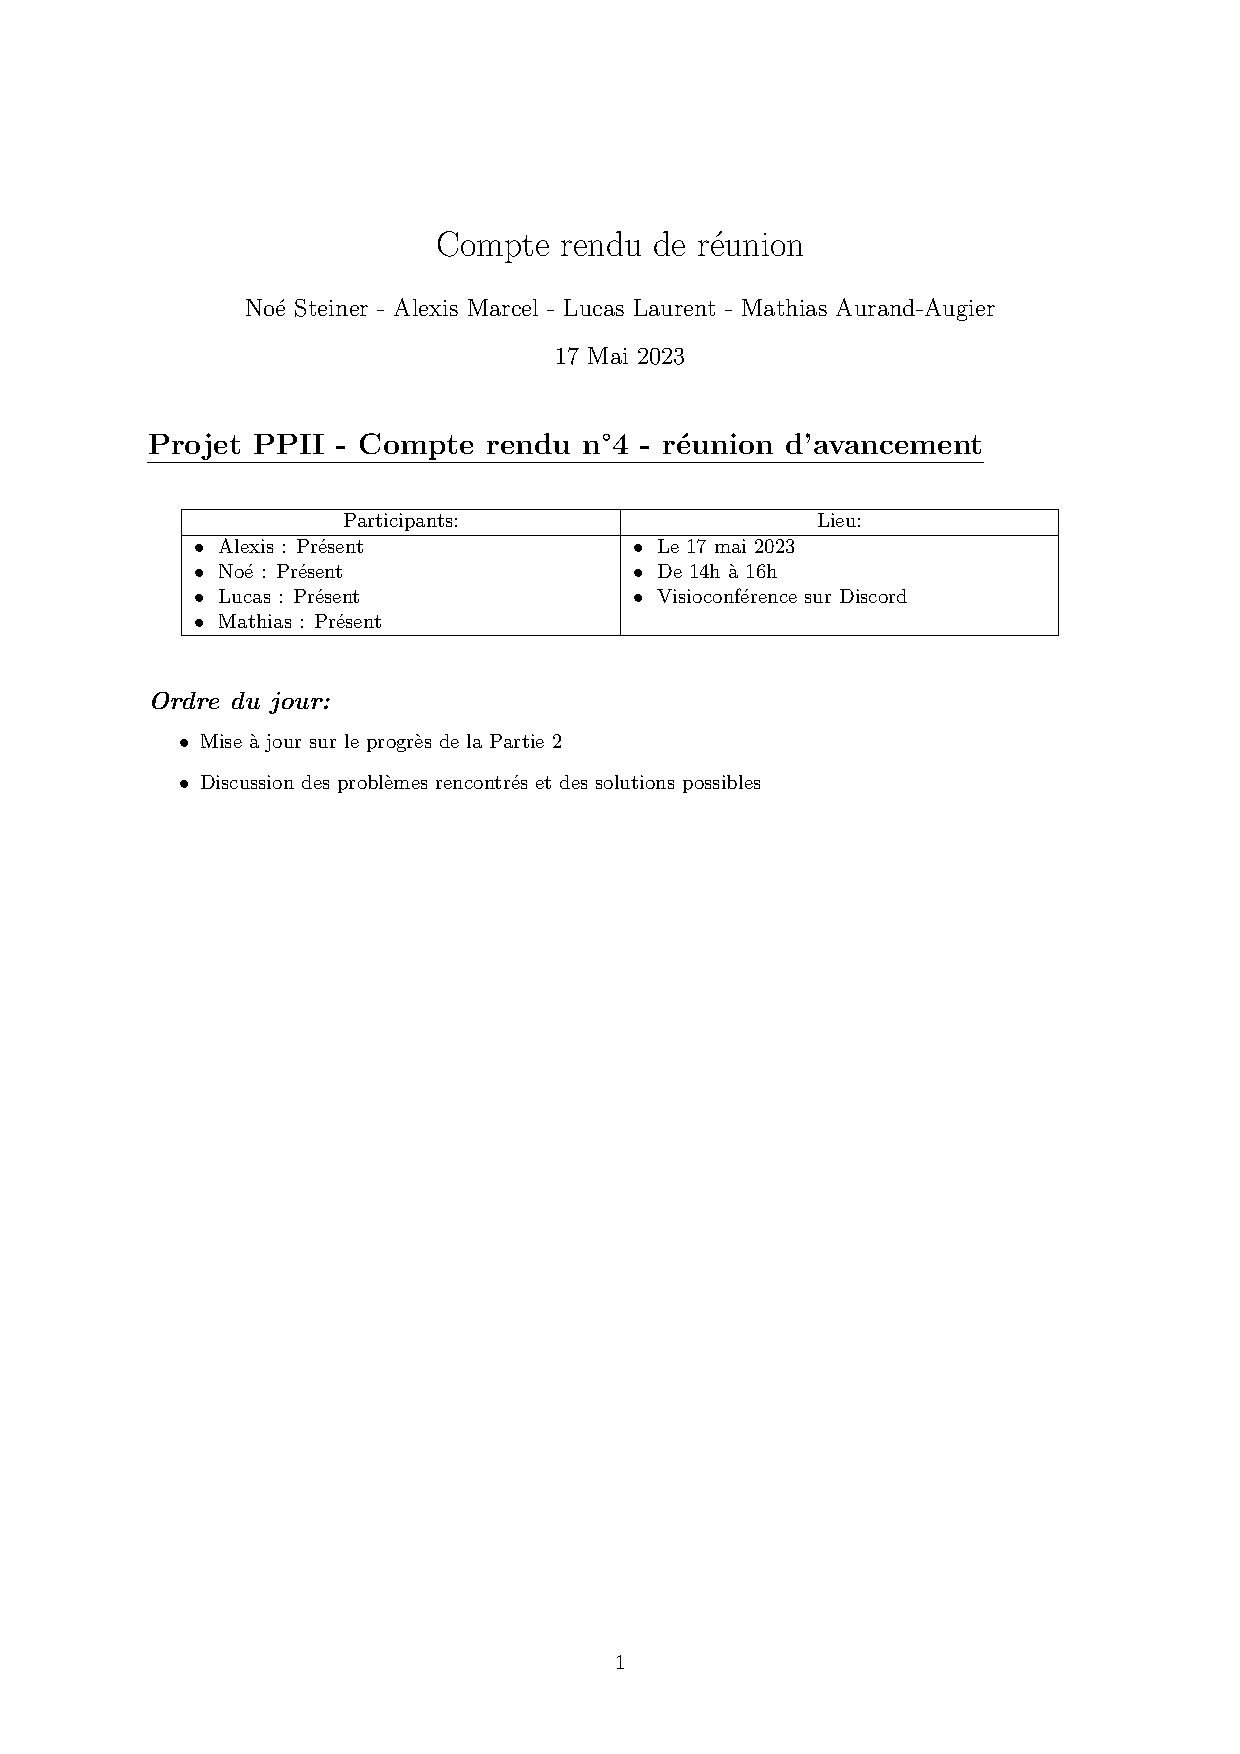
\includepdf[pages=1]{../cr_reu/reu4/cr_reu4.pdf}
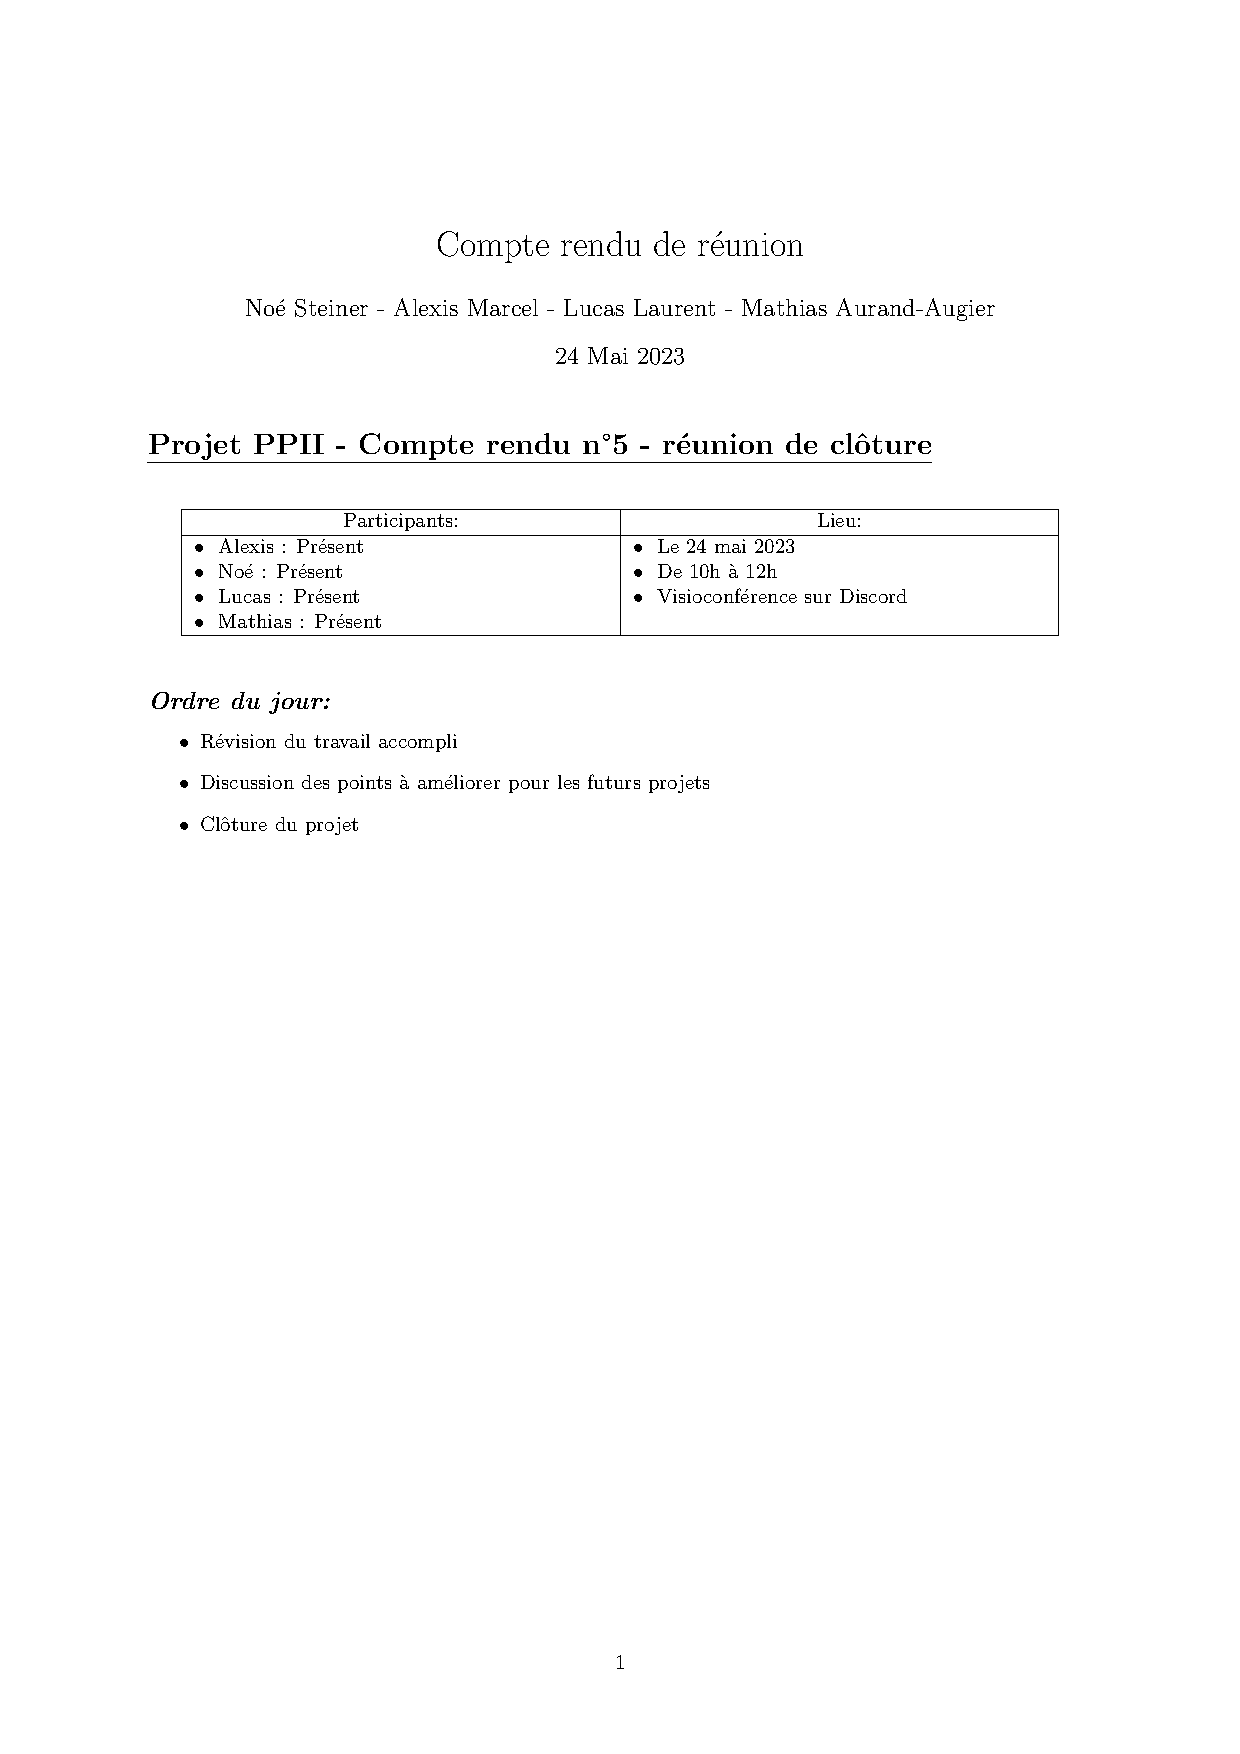
\includepdf[pages=1]{../cr_reu/reu5/cr_reu5.pdf}
\end{document}